\documentclass[a4paper, 12pt, notitlepage]{report}

\usepackage[T1]{fontenc}
\usepackage{textcomp}
\usepackage{xfrac}
\usepackage{bm}

\usepackage[utf8]{inputenc}
\usepackage[english,italian]{babel}
\usepackage{verbatim}
\usepackage{listings}

\usepackage{hyperref}
\usepackage{etoc}

\usepackage{float}
\usepackage{amsmath}
\usepackage{amsthm}
\usepackage{amsfonts}
\usepackage{mathtools}

\usepackage{fancyvrb}

\usepackage{xargs}
\usepackage[pdftex,dvipsnames,table,xcdraw]{xcolor}

\usepackage{xcolor}

% Package per il plot dei diagrammi di Bode
\usepackage{tikz}
\usetikzlibrary{calc}
\usetikzlibrary{arrows}
\usepackage{pgfplots}


\usepackage{graphicx} % graphics package
\usepackage{subcaption}
\graphicspath{ {./media/} } % images folder path


\usepackage{geometry}
\geometry{
    a4paper,
    top=30mm,
    bottom=30mm,
    left=35mm,
    right=35mm
}

\usepackage[pagestyles]{titlesec}
\titleformat{\chapter}[display]{\normalfont\bfseries}{}{0pt}{\Huge}

\newpagestyle{main}{
    \sethead[\thepage][][\chaptertitle]
        {}{}{\thepage}
    \setfoot[][][]
        {}{}{}
}

\usepackage[section]{placeins} % utilizzare /FloatBarrier alla fine della definizione delle figure per non farle scivolare in altre sezioni o altro

\usepackage{wrapfig} %Viene utilizzato per scrivere intorno alle immagini

\renewcommand*\contentsname{Index}

% remove new paragraph indentation
\setlength{\parindent}{0cm}

% colors for code snippets
\definecolor{codegreen}{rgb}{0,0.7,0.5}
\definecolor{codegray}{rgb}{0.5,0.5,0.5}
\definecolor{codeblue}{rgb}{0,0.5,0.82}
\definecolor{backcolour}{rgb}{0.95,0.95,0.95}

\lstdefinestyle{main}{
    backgroundcolor=\color{backcolour},
    commentstyle=\color{codegreen},
    keywordstyle=\color{orange},
    numberstyle=\tiny\color{codegray},
    stringstyle=\color{codeblue},
    basicstyle=\ttfamily\footnotesize,
    breakatwhitespace=false,
    breaklines=true,
    captionpos=b,
    keepspaces=true,
    numbers=left,
    numbersep=5pt,
    showspaces=false,
    showstringspaces=false,
    showtabs=false,
    tabsize=2
}
\lstset{style=main}

\newtheoremstyle{thmstyle}
	{\topsep}% measure of space to leave above the theorem. E.g.: 3pt
	{\topsep}% measure of space to leave below the theorem. E.g.: 3pt
	{}% name of font to use in the body of the theorem
	{}% measure of space to indent
	{\bfseries}% name of head font
	{ }% punctuation between head and body
	{.1em}% space after theorem head; " " = normal interword space
	{\thmname{#1}}% Manually specify head
\theoremstyle{thmstyle}

\newtheorem{example}{Example}



% front page created with \title command
\title{
    \includegraphics[scale=0.2]{unilogo.png}
    
    \vspace{1cm}{
        \large{\textbf{UNIVERSIT\`{A} DEL SALENTO}}
    }
        
    %\normalfont{Relazione di Laboratorio}
    \par\noindent\rule{\textwidth}{0.4pt}
    
    \vspace{0.3cm}
    \small{Mirko Caforio, Alessandro Convertino, Raffaele Crusi, Federico Izzi, Giovanni Pepe, Matteo Rosato, Antonio Scelsi, Ludovico Scurti}
    
    \vspace{1.0cm}
    \Large{Relazione di laboratorio: Misure su componenti e circuiti tramite strumentazione}
    
    \vspace{4.0cm}
    
    \par\noindent\rule{\textwidth}{0.4pt}
    \vspace{0.3cm}
    
    \small{ACADEMIC YEAR 2022/2023}
    \thispagestyle{empty}
}

\author{}
\date{}

\hypersetup{hidelinks}


\begin{document}
    % front page creation
    \maketitle
    \thispagestyle{empty}

    % blank page
    \newpage
    \mbox{}
    \thispagestyle{empty}
    
    % index creation
    \hypersetup{hidelinks}
    \tableofcontents
    \addtocontents{toc}{\protect\thispagestyle{empty}}
    \thispagestyle{empty}

    % Chapter: "Introduction"
    \hypersetup{hidelinks}
    \chapter{Introduzione}
\label{chap:introduction}

Durante il corso di "Fondamenti di Misure", abbiamo potuto effettuare 3 diverse esperienze di laboratorio.

\vspace{5mm}
Le esperienze si componevano di una prima parte in laboratorio in cui abbiamo effettivamente utilizzato gli strumenti e effettuato le dovute misurazioni.

La seconda parte invece riguardava lo studio dell'esperienza appena svolta e dei dati ottenuti, la valutazione delle incertezze delle varie misure effettuate e la stesura della relazione.

\vspace{5mm}

Nei seguenti 3 capitoli, tali esperienze sono descritte in maniera dettagliata, con la spiegazione di tutti i procedimenti seguiti, la teoria alla base delle operazioni svolte e la presentazione in forma tabellare dei dati raccolti ed elaborati.

    % Chapter 2
    \hypersetup{hidelinks}
    \chapter{Misure di Resistenza ed Impedenza con DMM e LCR}
\label{chap:prima_prova}


\section*{Obiettivo}
\label{sec:ob_first}

L'obiettivo primario di questa iniziale esperienza di laboratorio consiste nell'acquisire familiarità con l'utilizzo di strumentazione di base per le misurazioni, con le corrette procedure di misurazione e con la valutazione dell'incertezza associata, nel caso di misurazioni di resistenza e impedenza.
\newline \newline
A tale scopo ci è stato dato un resistore dal valore nominale di 1,5 $\Omega$ (valore nominale apprezzabile ad occhio nudo, tramite la visualizzazione delle lineette di colore marrone, verde, oro (vedi figura \ref{fig:resistore})) con un incertezza del 5\% (dato che l'ultimo anello è di colore oro).

\begin{figure}[h]
    \centering
    \includegraphics[height=10cm]{resistoretab.png}
    \caption{Tabella che raffigura il codice dei colori di un resistore}
    \label{fig:resistore}
\end{figure}
\FloatBarrier
\clearpage




\section{Misure di resistenze con multimetro portatile}
\label{sec:mult_port}

\begin{figure}[h]
    \centering
    \includegraphics[height=10cm]{multimetro_port.png}
    \caption{Multimetro utilizzato (Hewlett Packard 974A)}
    \label{fig:multimetro_port}
\end{figure}
\FloatBarrier

Il multimetro HP 974A è dotato di un display a 4 ½ cifre, il quale rappresenta uno strumento con 4 cifre principali e un'ulteriore cifra riservata per indicare il segno e, eventualmente, il valore della cifra più significativa della misurazione. Per calcolare la resistenza con un valore nominale dichiarato dal produttore pari a (1500 ± 75) m$\Omega$, abbiamo utilizzato il pulsante "RANGE" per impostare il valore di fondo scala, ovvero il limite superiore che il multimetro può "misurare", a 500 $\Omega$. Dato che lo strumento ha un campo di misura pari a 1/50000 del valore di fondo scala, il passo di quantizzazione, indicato come "Q", è pari a
\begin{equation}
    Q = \frac{V_{F_S}}{50000} = \frac{500}{50000} = 10 m\Omega
\end{equation}
con un incertezza di quantizzazione pari a: 
\begin{equation}
    U_q = \frac{Q}{2} = 5 m\Omega
\end{equation}

Procediamo con la valutazione dell'incertezza di \textbf{tipo B}, basata sull'utilizzo di informazioni note a priori quali le specifiche metrologiche degli strumenti adoperati. L’incertezza del dispositivo è data da una formula binomia composta da una parte proporzionale alla lettura e da un’altra pari a un numero fisso di LSB, quindi 
 proporzionale alla portata. Le specifiche del costruttore dello strumento, per misure di resistenze, sono le seguenti:

\begin{figure}[h]
    \centering
    \includegraphics[height=4cm]{incertezza_port.png}
    \caption{Specifice di incertezza dello strumento utilizzato (Hewlett Packard 974A)}
    \label{fig:Incertezza_multimetro_port}
\end{figure}
\FloatBarrier

Avendo impostato un valore di fondo scala pari a 500 $\Omega$ possiamo notare dalla precedente tabella un’incertezza pari a ±(0,06\% + 2) $\Omega$ , dove il primo termine è proporzionale alla lettura e il secondo alla portata. Si noti che per misure di ampiezza è possibile definire un modello semplificato di uno strumento per misure statiche, del tipo:

\begin{figure}[h]
    \centering
    \includegraphics[height=3cm]{modello_semplificato.png}
    \label{fig:modello}
\end{figure}
\FloatBarrier

Su cui definiamo un errore totale sulla misura del tipo:

\begin{equation}
    E_t(x) = \Delta Gx + O + inl(x) + e_q(g(x)) + N
\end{equation}

%\begin{figure} [h]
%    \centering
%    \includegraphics[height=2cm]{errore_port.png}
%    \label{fig:errore port}
%\end{figure}

Attraverso una serie di passaggi otteniamo l'incertezza come:
\begin{equation}
    |E_t| = |y_q - x| = | \Delta Gx + O + inl(x) + e_q(g(x)) | \leq 
\end{equation}
applichiamo una disuguaglianza triangolare
\begin{equation*}
    \leq | \Delta Gx | + | O | + | inl(x) | + | e_q(g(x)) | \leq 
\end{equation*}
applichiamo una disuguaglianza errore-incertezza
\begin{equation*}
    \leq U_G|x| + U_o + U_{inl} + U_q \cong U_G|y_q| + U_o + U_{inl} +U_q = U_{tot}
\end{equation*}

Dove, ipotizzando di unire l'incertezza di non linearità integrale nell'incertezza di portata, posso scrivere $U_g$ (incertezza di guadagno), $U_o$ (incertezza di portata dell'offset) e $U_q$ (incertezza di quantizzazione) come: 
\begin{equation}
\left\{\begin{array}{l}
    | \Delta G \cdot y_q | \leq U_G |y_q| \ , \ con \ U_g=0,06\% \\
| O + inl(x) + e_q(g(x)) | \leq U_{o+inl+q} \ , \ con \ U_{o+inl+q}=2LSB
\end{array}\right.
\end{equation}

Quindi, chiamando Q, passo di quantizzazione e $V_L$ valore letto (supponiamo di usare il primo valore letto nella tabella \label{mult_port}):

\begin{equation*}
\begin{array}{l}
U(R) = U_G \cdot V_L + U_{o+inl+q} \cdot Q = 0,06\% \cdot 1,62\Omega + 2 \cdot 0,01 \Omega \\ \\
= (0,972 + 20) m\Omega = 0,02 \Omega
\end{array}
\end{equation*}

sapendo che possiamo esprimere la resistenza misurata $R_M$ e il range della resistenza r(R) per la prima misurazione effettuata come:
\begin{equation*}
    R_M = (1,62 \pm 0,02) \Omega
\end{equation*}
\begin{equation*}
    r(R) = [1,60 \Omega \div 1,64 \Omega]
\end{equation*}

Va notato che l'inclusione dell'errore di non linearit\'a integrale nel secondo termine dell'incertezza fornita dal produttore ( proporzionale alla portata) rende tale termine non solamente un errore di offset puro, ma include anche l'errore di quantizzazione. Pertanto, nel caso di differenze tra misurazioni, non possiamo semplicemente sottrarre l'errore di offset.

\begin{comment}
Notiamo, usando la resistenza nominale di $(1500 \pm 7,5) m\Omega$ e graficandola con la (2.9) che i due range di valori non sono compatibili.

\begin{figure}[h]
    \centering
    \includegraphics[height=4cm]{range.png}
    \caption{Differenza dei due range}
    \label{fig:range}
\end{figure}
\FloatBarrier
\end{comment}

\vspace{5mm}
La misura eseguita utilizzando il multimetro portatile fornisce una stima non corretta del valore della resistenza. Inoltre, lo strumento non consente la compensazione degli errori sistematici poiché non dispone di funzioni di calibrazione. Infine, non si è tenuto conto degli errori dovuti alle resistenze di contatto tra i cavi, i puntali e il resistore. Il contributo di tutti questi effetti influisce sul risultato finale della misura.

Se vogliamo quantificare l'accuratezza della prima misura, assumiamo come valore "vero" della grandezza misurata il valore nominale della resistenza. Facendo questa assunzione, possiamo ottenere una stima dell'errore sistematico come differenza tra il risultato della misura e il valore nominale del componente misurato:
\begin{equation}
    E_S = 1,62 - 1,50 = 0,12\Omega
\end{equation}
L’accuratezza relativa “a” di una misura può essere espressa in funzione di tale errore 
stimato in errore relativo mediante la seguente espressione: 
\begin{equation}
     a = 1 - \left| \frac{E_S}{R_{NOMINALE}}\right| = 92\%
\end{equation}
\clearpage

\subsection*{La nostra prova}
\label{sub:nosta_prova_first}

\vspace{0.5cm}
%\begin{wrapfigure}{l}{0.3\textwidth}
\FloatBarrier
%\begin{figure}[h]
\begin{wrapfigure}{r}{0.3\textwidth}
    \centering
    \includegraphics[width=0.25\textwidth]{Gameboy_62.jpg}
    \label{fig:mult_port_nostro}
\end{wrapfigure}
%\end{figure}
\FloatBarrier
%\end{wrapfigure}
    
Quando usiamo il multimetro portatile abbiamo disposto i puntali in maniera pi\'u stabile possibile, applicando una buona pressione per ottenere una misurazione pi\'u fedele possibile,
Abbiamo fatto 10 ripetizioni in modo da ricavare l'incertezza totale, con il contributo valutato di tipo B relativamente alla specifica di strumento utilizzato.
\newline
\newline
Con i valori ottenuti (\ref{tab:mult_port}) eseguiamo una valutazione di tipo A, dove il risultato di misura sarà dato dalla media delle misure in un range di incertezza pari dalla deviazione standard. Ovviamente poich\'e stiamo utilizzando un numero finito e relativamente piccolo di misure otteniamo solo una stima della media statistica, che idealmente (numero infinito di misure) rappresenta il valore vero del misurando. Quindi calcoliamo la media e la varianza campionarie sfruttando il campione di misure (\ref{tab:mult_port}):
\begin{align*}
    \mu_{10}=\frac{1}{N}\sum_{i=1}^{10}R_{i}=1,61\Omega
\end{align*}
\begin{equation*}
    u_{10}=\sqrt{\frac{1}{9}\sum_{i=1}^{10}(R_i-\mu_{10})^{2}}=0,008\Omega 
\end{equation*}
\FloatBarrier

\begin{table}[!ht]
    \centering
    \caption{Multimetro portatile 974A, fondo scala di 500 $\Omega$}
    \begin{tabular}{|c|c|c|c|}
    \hline
        \textbf{R}$\bm{[\Omega]}$ & \textbf{Q}$\bm{[\Omega]}$ & \textbf{Uq} $\bm{[\Omega]}$ & $\bm{U_r}$ \\ \hline
        1,62 & 0,01 & 0,01 & 0,02  \\ \hline
        1,61 & 0,01 & 0,01 & 0,02  \\ \hline
        1,61 & 0,01 & 0,01 & 0,02  \\ \hline
        1,62 & 0,01 & 0,01 & 0,02  \\ \hline
        1,60 & 0,01 & 0,01 & 0,02  \\ \hline
        1,60 & 0,01 & 0,01 & 0,02  \\ \hline
        1,62 & 0,01 & 0,01 & 0,02  \\ \hline
        1,61 & 0,01 & 0,01 & 0,02  \\ \hline
        1,60 & 0,01 & 0,01 & 0,02  \\ \hline
        1,61 & 0,01 & 0,01 & 0,02 \\ \hline
    \end{tabular}
    
    \label{tab:mult_port}
\end{table}
\FloatBarrier
\clearpage

%---------Multimetro da Banco---------%
\section{Misure di resistenza con multimetro da banco}
\label{sec:mult}


\begin{figure}[h]
    \centering
    \includegraphics[height=5cm]{mult_banco.png}
    \caption{Multimetro HP Hewlett Packard 34401A}
    \label{fig:mult_banco}
\end{figure}
\FloatBarrier

Per il calcolo della resistenza di valore nominale pari a (1500 ± 7,5) m$\Omega$, impostiamo la risoluzione dello strumento a 6 ½ cifre premendo sul tasto \emph{Shift} e poi sul tasto \emph{Auto/Man}. Successivamente impostiamo la portata dello strumento a 100,0000 $\Omega$ mediante gli appositi pulsanti della sezione \emph{RANGE/DIGITS}. In questo modo lo strumento ha un campo di misura 
pari a 1/1000000 del valore di fondo scala e quindi il passo di quantizzazione Q sar\'a: 
\begin{equation}
    Q = \frac{V_{FS}}{CM} = \frac{10^2}{10^6} = 0,0001 \Omega
\end{equation}
Con l'incertezza di quantizzazione $U_q$ pari a:
\begin{equation}
    U_q = \frac{Q}{CM} = 0,00005 \Omega
\end{equation}

Quando abbiamo lavorato con il multimetro da banco, abbiamo dapprima lavorato in modalità "2 terminali" (attivata premendo su  \emph{$\Omega$2W} che ci permette di lavorare a due morsetti).

\begin{figure}[h]
    \centering
    \includegraphics[height=2cm]{mult_banco_zoom.png}
    \caption{Zoom sui tasti premuti}
    \label{fig:mult_banco_zoom}
\end{figure}
\FloatBarrier

Come prima operazione abbiamo cortocircuitato i morsetti, premendo il tasto null, in modo che il valore di resistenza interna del conduttore dei cavi venga preso in considerazione permettendoci di tarare lo strumento, mostrando una misurazione prossima a zero (nel nostro caso abbiamo visualizzato a display, impostato a 6 cifre e mezzo, il valore 0,000134).

% L HO RIMOSSA MOMENTANEAMENTE PERCHE' NON MI PIACE LA IN MEZZO TROPPO BIANCO
%\begin{figure}[h]
%    \centering
%    \includegraphics[height=4cm]{2Morsetti_432.jpg}
%    \label{fig:2morsetti}
%\end{figure}
%\FloatBarrier

\'E importante notare che se la resistenza dei cavi è comparabile o superiore alla resistenza che si desidera misurare, il risultato della misura potrebbe essere influenzato significativamente dal contributo della resistenza dei cavi, dunque per ridurre gli errori sistematici:
\begin{equation*}
    Risultato = Valore \ \ letto - Valore\ \ NULL
\end{equation*}

\begin{figure}[h]
    \centering
    \includegraphics[height=9cm]{tabella_mult_banco.png}
    \label{fig:tab_mult_banco}
\end{figure}
\FloatBarrier

Avendo impostato un valore di fondo scala pari a 100,0000 $\Omega$, in un ambiente con una temperatura pari a (23 $\pm$ 5)°C, facciamo riferimento all'incertezza $\pm$(0,010 $\% \pm 0,004 \%$), con il primo termine proporzionale alla lettura e il secondo proporzionale alla portata.
Ragionando come prima, ipotizzando di unire l'incertezza di non linearità integrale nell'incertezza di portata, posso scrivere $U_g$ (incertezza di guadagno), $U_o$ (incertezza di portata dell'offset) e $U_q$ (incertezza di quantizzazione) come: 
\begin{equation}
\left\{\begin{array}{l}
| \Delta G \cdot y_q | \leq U_G |y_q| \ , \ con \ U_g=0,01\% \\ 
| O + inl(x) + e_q(g(x)) | \leq U_{o+inl+q} \ , con \ U_{o+inl+q}=0,004\%
\end{array}\right.
\end{equation}
Quindi, chiamando P, portata e $V_L$ valore letto (supponiamo di usare il primo valore letto nella tabella \label{mult_port}):
\begin{equation*}
    U(R) = U_G \cdot V_L + U_{o+inl+q} \cdot P = 0,01\% \cdot 1,648\Omega + 0,004 \% \cdot 100 \Omega = 0,004 \Omega 
\end{equation*}

dove U(R) è stato arrotondato per difetto.

\begin{table}[!ht]
\resizebox{\textwidth}{!}{%
    \centering
    \begin{tabular}{|c|c|c|c|c|c|c|}
    \hline
        \textbf{R [$\bm{\Omega}$]} & \textbf{Fondo scala} $\bm{[\Omega]}$ & \textbf{Q} $\bm{[\Omega]}$ & $\bm{U_q\ \ [\Omega]}$ & $\bm{U_R}$ \textbf{[$\bm{\Omega}$]} \\ \hline
        1,648 & 100 & 0,0001 & 0,00005 & 0,0042 \\ \hline
        1,614 & 100 & 0,0001 & 0,00005 & 0,0042 \\ \hline
        1,627 & 100 & 0,0001 & 0,00005 & 0,0042 \\ \hline
        1,614 & 100 & 0,0001 & 0,00005 & 0,0042 \\ \hline
        1,432 & 100 & 0,0001 & 0,00005 & 0,0041 \\ \hline
        1,466 & 100 & 0,0001 & 0,00005 & 0,0041 \\ \hline
        1,441 & 100 & 0,0001 & 0,00005 & 0,0041 \\ \hline
        1,468 & 100 & 0,0001 & 0,00005 & 0,0041 \\ \hline
        1,475 & 100 & 0,0001 & 0,00005 & 0,0041 \\ \hline
        1,493 & 100 & 0,0001 & 0,00005 & 0,0041 \\ \hline
    \end{tabular}%
    }
    \caption{Multimetro 34401A (6$\sfrac{1}{2}$ cifre), 2 Morsetti, R (dei morsetti) = 0,133 $\Omega$}
    \label{tab:mult_2w}
\end{table}
\FloatBarrier
 Per il primo valore di resistenza misurata col multimetro è 1,648 $\Omega$, il risultato della misura si esprime come R=(+1,648 $\pm$ 0,004)$\Omega$.


\begin{figure}[h]
    \centering
    \includegraphics[height=5cm]{quattro_morsetti.png}
    \caption{Metodo Kelvin a 4 morsetti}
    \label{fig:quattro morsetti}
\end{figure}
\FloatBarrier



\begin{wrapfigure}{l}{0.3\textwidth}
    \centering
    \includegraphics[width=0.28\textwidth]{4Morsetti_472.jpg}
    \label{fig:4morsetti}
\end{wrapfigure}
\FloatBarrier
Successivamente, sempre con lo stesso multimetro da banco, abbiamo lavorato in modalità "4 terminali" (attivata premendo su \emph{Shift}, e poi successivamente su \emph{$\Omega$2W} per lavorare a quattro morsetti).


Anche in questo caso abbiamo nuovamente cortocircuitato i morsetti, premendo nuovamente il tasto null per tarare lo strumento e riavere un valore associato al cortocircuito pi\'u prossimo allo zero possibile in presenza del cortocircuito (nel nostro caso 0,004).


Attraverso la prima coppia di morsetti (Hi, Lo), lo strumento inietta la corrente nota come "$I_0$" nella resistenza. Questa corrente attraversa le boccole (Hi, Lo) dove si incontra con la resistenza di contatto, che può falsare la misura standard a due fili (impostando $\Omega$2W sul pannello frontale del multimetro).

Per evitare questo problema, tramite l'altra coppia di morsetti di sensing (Hi, Lo), viene prelevata la tensione su due punti più vicini al resistore. Utilizzando questa configurazione (impostando $\Omega$4W sul pannello frontale del multimetro), le cadute di tensione sulle resistenze di contatto presenti sulle boccole che portano la corrente al resistore in prova possono essere escluse dalla tensione da misurare, garantendo una misurazione più accurata.

Si effettua l'operazione di NULL in modo analogo al caso precedente, misurando un valore di resistenza pari a R = 1,478 $\Omega$. Dalla teoria, questo valore dovrebbe essere più accurato rispetto al caso del multimetro a due morsetti. Utilizzando il modello precedente per il calcolo dell'incertezza, otteniamo:

\begin{equation}
    \left\{\begin{array}{l}
| \Delta G \cdot y_q | \leq U_G |y_q|,    con U_g=0,01\%
\\ | O + inl(x) + e_q(g(x)) | \leq U_{o+inl+q}, con U_{o+inl+q}=0,004\%
\end{array}\right.
\end{equation}


    


Quindi, chiamando P, portata e $V_L$ valore letto (supponiamo di usare il primo valore letto nella tabella \label{mult_port}):

\begin{equation*}
    U(R) = U_G \cdot V_L + U_{o+inl+q} \cdot P = 0,01\% \cdot 1,478\Omega + 0,004 \% \cdot 100 \Omega = 0,004 \Omega 
\end{equation*}
(dove il risultato è stato arrotondato per difetto)
Notiamo che l’incertezza in questo caso non è cambiata, con R=(+1,478 $\pm$ 0,004)$\Omega$



\begin{table}[!ht]
\resizebox{\textwidth}{!}{%
    \centering
    \begin{tabular}{|c|c|c|c|c|c|c|}
    \hline
        \textbf{R [$\bm{\Omega}$]} & \textbf{Fondo scala} $\bm{[\Omega]}$ & \textbf{Q} $\bm{[\Omega]}$ & $\bm{U_q\ \ [\Omega]}$ & $\bm{U_R}$ \textbf{[$\bm{\Omega}$]} \\ \hline
        1,478 & 100 & 0,0001 & 0,00005 & 0,0042 \\ \hline
        1,478 & 100 & 0,0001 & 0,00005 & 0,0042 \\ \hline
        1,478 & 100 & 0,0001 & 0,00005 & 0,0042 \\ \hline
        1,478 & 100 & 0,0001 & 0,00005 & 0,0042 \\ \hline
        1,478 & 100 & 0,0001 & 0,00005 & 0,0042 \\ \hline
        1,478 & 100 & 0,0001 & 0,00005 & 0,0042 \\ \hline
        1,478 & 100 & 0,0001 & 0,00005 & 0,0042 \\ \hline
        1,478 & 100 & 0,0001 & 0,00005 & 0,0042 \\ \hline
        1,478 & 100 & 0,0001 & 0,00005 & 0,0042 \\ \hline
        1,478 & 100 & 0,0001 & 0,00005 & 0,0042 \\ \hline
    \end{tabular}%
    }
    \caption{Multimetro 34401A (6$\sfrac{1}{2}$ cifre), 4 Morsetti, R (dei morsetti) = 0,004 $\Omega$}
    \label{tab:mult_4w}
\end{table}
\FloatBarrier


Volendo quantificare gli errori sistematici:
\begin{equation*}
    E_{S(2W)} = 1,529 - 1,500 = 0,029 \Omega
\end{equation*}
\begin{equation*}
   | E_{S(4W)} | = | 1,478 - 1,500 | = 0,022 \Omega
\end{equation*}
che portano alle seguenti accuratezze: 
\begin{align*}
a_{2W} = 1 - \left| \frac{E_{S(2W)}}{R_{NOMINALE}} \right| = 98\%
   &&   
a_{4W} = 1 - \left| \frac{E_{S(4W)}}{R_{NOMINALE}} \right| = 98,5\%
\end{align*}

\begin{comment}
\begin{figure}[h]
    \centering
    \includegraphics[height=3cm]{banco_misure.png}
    \label{fig:range}
\end{figure}
\FloatBarrier
\end{comment}

Osserviamo questa volta che utilizzando il multimetro da banco a 6 ½ cifre si ottiene una stima più precisa del valore misurato rispetto all'utilizzo del multimetro portatile descritto precedentemente. Questi miglioramenti possono essere attribuiti alla capacità dello strumento da banco di ridurre gli errori sistematici mediante l'implementazione di funzioni adeguate.

Il multimetro da banco a 6 ½ cifre offre una maggiore precisione grazie alla sua elevata risoluzione e alla possibilità di compensare gli errori sistematici tramite funzioni avanzate di calibrazione e correzione. Ciò consente di ottenere misurazioni più accurate e affidabili, riducendo l'effetto degli errori di offset, delle non linearità e di altri fattori che potrebbero influenzare la precisione della misura.

Inoltre, lo strumento da banco può offrire un controllo più preciso delle condizioni operative, come la compensazione della resistenza dei cavi o la selezione della modalità di misura più adatta alle specifiche dell'applicazione. Ciò contribuisce ulteriormente a migliorare l'accuratezza complessiva della misurazione.

E osserviamo ciò calcolando l'incertezza valutata di tipo A sfruttando prima il campione di misure ottenuto lavorando con due morsetti (\ref{tab:mult_2w}) :

\begin{align*}
    \mu_{10}=\frac{1}{N}\sum_{i=1}^{10}R_{i}=1,529\Omega  &&  u_{10}=\sqrt{\frac{1}{9}\sum_{i=1}^{10}(R_i-\mu_{10})^{2}}=0,086\Omega 
\end{align*}
\FloatBarrier

e poi lavorando con quattro morsetti (\ref{tab:mult_4w}):

\begin{align*}
    \mu_{10}=\frac{1}{N}\sum_{i=1}^{10}R_{i}=1,478\Omega && u_{10}=\sqrt{\frac{1}{9}\sum_{i=1}^{10}(R_i-\mu_{10})^{2}}=0\Omega 
\end{align*}
\FloatBarrier

Concludiamo che, usando una resistenza con valore nominale di (1500 ± 7,5) m$\Omega$, con il multimetro da banco otteniamo una stima pari a R=(+1,529 $\pm$ 0,086)$\Omega$ per la misurazione a due morsetti, mente otteniamo una stima pari a R=(+1,478 $\pm$ 0)$\Omega$ per la misurazione a 4 morsetti.
\clearpage

%----------LCR-----------%
\section{Misure con LCR-Meter}
\label{sec:lcr}

\subsection{Strumentazione}
\label{sub:strum}
Lo scopo dell’esercitazione è quello di effettuare misure di impedenze per mezzo 
dell’LCR-meter e di valutare l’incertezza di tali misure facendo uso delle specifiche 
del costruttore, cioè eseguendo valutazioni dell’incertezza di tipo B.
Il disegno illustrativo del montaggio dell’apparecchiature è il seguente:

\begin{figure}[h]
    \centering
    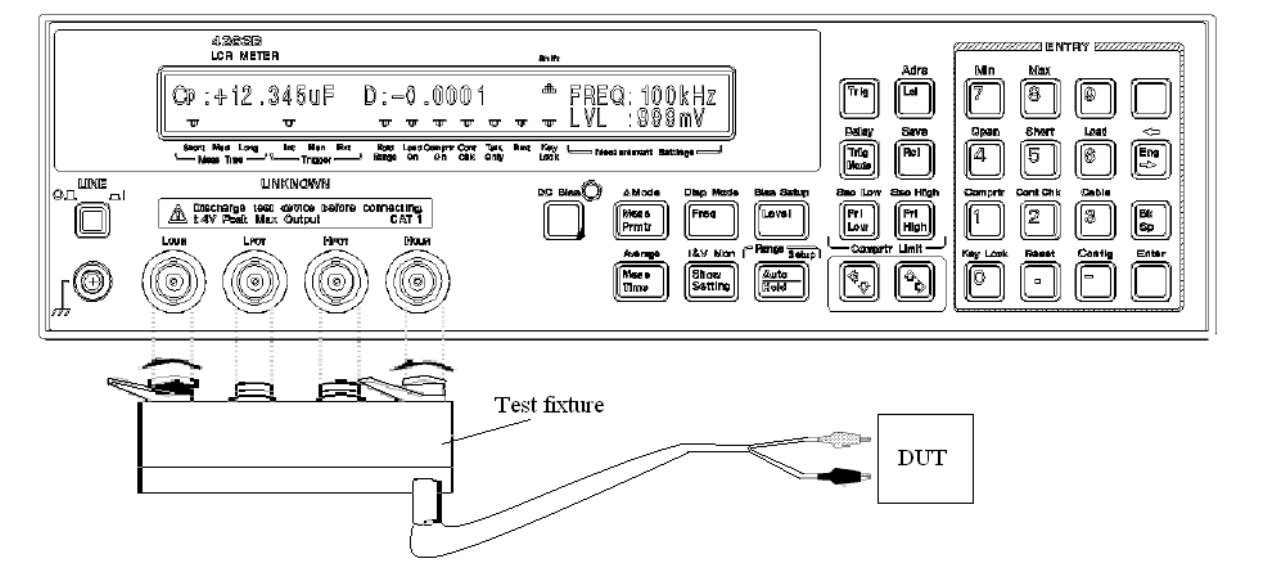
\includegraphics[height=6cm]{media/LCR_meter.png}
    \label{fig:LCR_meter}
\end{figure}
\FloatBarrier

\begin{itemize}
    \item AGILENT LCR-meter 4263B;
    \item Kelvin clip leads di lunghezza pari a 1m;
    \item Test fixture;
    \item Resistenza con valore nominale pari a $(1000\pm50)m\Omega$;
    \item Capacità con valore nominale pari a $(6800\pm340)pF$;
\end{itemize}


I seguenti strumenti consentono di determinare i parametri di induttanza, capacità, resistenza, fattore di merito e coefficiente di perdita per induttori, condensatori e resistori, utilizzando gli schemi equivalenti prefissati degli oggetti sottoposti ad analisi.

L'oggetto in prova viene sottoposto a basse tensioni e correnti durante il test, con un livello di segnale che può essere regolato dall'operatore da alcuni millivolt a 1 volt efficace, quando si lavora a tensione fissa.

Il tempo trascorso tra l'inizio di una misura e l'inizio della successiva è di circa qualche decina di millisecondi e varia in base all'incertezza richiesta. Più piccola è l'incertezza richiesta, maggiore sarà il tempo necessario per la misurazione. Un esempio di valore possibile è 25 ms (short).

L'esercitazione è iniziata con il ripristino dei valori predefiniti del dispositivo e il collegamento del supporto di test al pannello frontale come mostrato nello schema di montaggio. Successivamente, possiamo procedere con la calibrazione dello strumento al fine di ridurre al minimo gli errori sistemici che possono influire sulle misurazioni.

Per evitare gli errori di sfasamento causati dalla lunghezza del cavo, abbiamo impostato la lunghezza del cavo a un metro utilizzando il comando corrispondente nel pannello frontale dell'LCR.

\begin{figure}[ht]
    \centering
    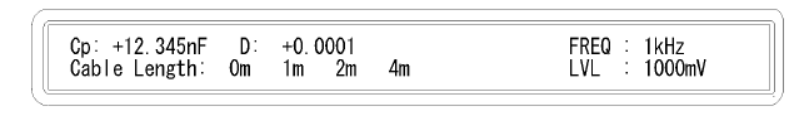
\includegraphics[height=2cm]{media/pannello_frontale_LCR.png}
    \caption{Pannello Frontale LCR}
    \label{fig:pannello_frontale_LCR}
\end{figure}
\FloatBarrier

Successivamente, abbiamo proceduto con la correzione OPEN/SHORT dello strumento
impostando prima la frequenza dell'LCR a 1KHz, alla quale eventuali variazioni delle condizioni operative dello strumento, come temperatura e umidità, potrebbero influire negativamente sull'incertezza della misura. Abbiamo poi lasciato i morsetti scollegati, in circuito aperto, premuto sul bulsante di colore blu, poi sul pulsante \emph{4}, su \emph{ENTER} e abbiamo infine atteso il messaggio "Open correction complete" sullo schermo. Abbiamo proseguito cortocircuitando i due morsetti, l'uno con l'altro, premuto il tasto di colore blu, seguito dal testo \emph{5}, dal pulsante \emph{ENTER} e abbiamo atteso la comparsa del messaggio "Short correction complete" sullo schermo.
 

\subsection{Impedenze}
\label{sub:z}

Tramite l'LCR-Meter abbiamo svolto l'ultima parte della nostra prima esperienza.

Di solito, per effettuare misurazioni di impedenza, è necessario stabilire un piano di riferimento sull'ingresso del DUT (Device Under Test) nel pannello frontale. L'LCR ci permette di fare ciò fissando la lunghezza del cavo utilizzato. Tuttavia, è importante cercare di eliminare le impedenze residue causate dalla presenza del Test Fixture nel pannello frontale dello strumento.

Per fare la prova, abbiamo impostato un tempo di misura medio LONG, premendo sul pulsante \emph{Meas Time} e selezionando LONG.
Per impostare i parametri da visualizzare per la resistenza abbiamo premuto su \emph{Meas Prmtr}, selezionato il primo parametro R, premuto \emph{ENTER}, selezionato il secondo parametro X e infine premuto nuovamente ENTER.
Partendo da una frequenza di 100Hz, abbiamo misurato la resistenza (R) e reattanza (X, nel nostro caso leggermente negativà perché prevale l'effetto induttivo). Abbiamo così calcolato tutti i valori al variare della frequenza, come mostrato nella seguente tabella.  


\begin{table}[!ht]
\centering
\begin{tabular}{|c|c|c|}
\hline
\textit{\textbf{Frequenza}} \textbf{[Hz]} & \textbf{R [$\bm{\Omega}$]}  & \textbf{X [m$\bm{\Omega}$]}  \\ \hline
100Hz                       & 1,4630    & -0,04      \\ \hline
120Hz                       & 1,4628    & -0,05      \\ \hline
1kHz                        & 1,4625    & -0,52      \\ \hline
10kHz                       & 1,4622    & -5,12      \\ \hline
100kHz                      & 1,4635    & -51,50     \\ \hline
\end{tabular}
\caption{LCR, misura Impedenza, Tempo di misura: Long}
\label{tab:lcr_z}
\end{table}
\FloatBarrier


Se rappresentiamo le precedenti misure in modulo e fase avremo i grafici nelle figure ~\ref{fig:modulo} e ~\ref{fig:fase}.
%Mancano i due grafici relativi a questa tabella%
%\begin{figure}[ht]
%    \centering
%    \includegraphics[height=2cm]{media/grafico_modulo.png}
%    \caption{Grafico del modulo}
%    \label{fig:grafico_modulo}
%\end{figure}
%
%\begin{figure}[ht]
%    \centering
%    \includegraphics[height=2cm]{media/grafico_fase.png}
%    \caption{Grafico della fase}
%    \label{fig:grafico_fase}
%\end{figure}

% Diagramma di Bode del modulo
\begin{figure}[h]
    \centering
    \resizebox{1\textwidth}{!}{%
    \begin{tikzpicture}
        \begin{axis}
            [xlabel={Frequenza [Hz]}, ylabel={|Z| [$\Omega$]},  ytick= {1.463000001, 1.462800001, 1.462500092, 1.462208964, 1.464405852},
             yticklabels= {1.4630, 1.4628, 1.4625, 1.4622, 1.4644}],
            \addplot[red, mark=*]
            table[x=x, y=y, col sep=comma] {media/bode/bode_modulo_1prova.txt};
        \end{axis}
    \end{tikzpicture}
    }%
    \caption{Diagramma di Bode del modulo di Z}
    \label{fig:modulo}
\end{figure}
\FloatBarrier
\clearpage

% Diagramma di Bode della fase
\begin{figure}[h]
    \centering
    \resizebox{1\textwidth}{!}{%
    \begin{tikzpicture}
        \begin{axis}
            [xlabel={Frequenza [Hz]}, ylabel={Fase [rad]},
            height=15cm, width=10cm
            ]
            \addplot[red, mark=*]
            table[x=x, y=y, col sep=comma] {media/bode/bode_fase_1prova.txt};
        \end{axis}
    \end{tikzpicture}
    }%
    \caption{Diagramma di Bode della fase di Z}
    \label{fig:fase}
\end{figure}
\FloatBarrier
\clearpage

Dai grafici precedenti si può notare che alle alte frequenze è necessario considerare gli effetti parassiti della resistenza reale, che tendono ad aumentare il valore nominale della resistenza linearmente con la frequenza.

Il circuito equivalente prevede un'induttanza in serie alla resistenza e una capacità in parallelo alla serie RL. I valori delle impedenze parassite dipendono dalla tecnica di costruzione.

Alle basse frequenze, l'effetto della capacità e dell'induttanza può essere trascurato in quanto la capacità si comporta come un circuito aperto e l'induttanza come un cortocircuito. Aumentando la frequenza, la capacità tende ad abbassare il valore della resistenza, mentre l'induttore tende ad aumentarlo fino a quando, alla frequenza $1/2\pi\sqrt{LC}$, la coppia LC entra in risonanza compensandosi reciprocamente.

Per il calcolo dell'incertezza delle misure di resistenza e reattanza riportate nella tabella precedente, dobbiamo fare riferimento alle specifiche del costruttore. Per il calcolo dell'incertezza, è necessario applicare la seguente formula:

\begin{equation}
    A_e = A + \frac{BCZ_S}{|Z_X|} + \frac{D}{|Z_X|} + \frac{|Z_X|}{E} \hspace{0,8cm} con \hspace{0,2cm} |Z_X| \leq 100\Omega
\end{equation}

dove $Z_X$ è il valore misurato dell’impedenza Z. L’incertezza di $|Z|$ è uguale a quella di 
R e di X per cui, consultando le tabelle di incertezza fornite dal costruttore, avremo:


%TABELLA INCERTEZZA IMPEDENZA%
\begin{table}[!ht]
\centering
\begin{tabular}{|c|c|c|c|c|c|c|c|}
\hline
\textbf{A}      & \textbf{B}      & \textbf{C} & \textbf{D [$\bm{\Omega}$]} & \textbf{E [$\bm{\Omega}$]}  & $\bm{Z_s \ \ [\Omega]}$ & $\bm{Z_x \ \ [\Omega]}$ & $\bm{U_z}$ \textbf{(Ae)} \\ \hline
0,005  & 0,0009 & 1 & 0,01      & 280.000.000,00  & 1          & 1,4630     & 0,0125  \\ \hline
0,005  & 0,0009 & 1 & 0,01      & 280.000.000,00  & 1          & 1,4628     & 0,0125  \\ \hline
0,004  & 0,0003 & 1 & 0,0165    & 28.000.000,00  & 1          & 1,4625     & 0,0155  \\ \hline
0,004  & 0,0003 & 1 & 0,075     & 2.800.000,00  & 1          & 1,4622     & 0,0555  \\ \hline
0,0097 & 0,0011 & 1 & 0,75      & 280.000,00  & 1          & 1,4635     & 0,5229  \\ \hline
\end{tabular}
\caption{Tabella di incertezza fornita dal costruttore, con $U_z$ l'incertezza}
\label{tab:lcr_z_sheet}
\end{table}
\FloatBarrier

Con l'incertezza di quantizzazione $U_q$ pari a:
\begin{equation}
    U_q = \frac{Q}{CM} = 0,00005 \Omega
\end{equation}
\clearpage


%-------------Capacità----------- %
\subsection{Capacità}
\label{sub:c}
Come ultima parte della prova abbiamo misurato i valori di un condensatore.
Per impostare i primi 2 parametri da visualizzare per la capacità abbiamo premuto su \emph{Meas Prmtr}, selezionato Cp, premuto \emph{ENTER}, selezionato Rp e ripremuto \emph{ENTER}. Successivamente per calcolare l'ultimo parametro necessario abbiamo premuto Cp, seguito da \emph{ENTER}, selezionato D e infine ripremuto \emph{ENTER}
Questa procedura è stata quindi ripetuta per tutti i valori di frequenza (partendo da 100kHz, arrivando fino ai 100Hz).


\begin{table}[ht]
\centering
%\resizebox{\textwidth}{!}{%
\begin{tabular}{|c|c|c|c|}
\hline 
\textit{\textbf{Frequenza [Hz]}} & \textbf{Cp [F]} & \textbf{Rp [\bm{$\Omega$}]} & \textbf{D}  \\ \hline
100Hz                       & 6,98E-09    & 1,27E+08     & 0,0018     \\ \hline
120Hz                       & 6,88E-09    & 1,33E+08     & 0,0017      \\ \hline
1kHz                        & 6,96E-09    & 5,42E+06     & 0,0039      \\ \hline
10kHz                       & 6,89E-09    & 2,60E+05     & 0,0095      \\ \hline
100kHz                      & 6,70E-09    & 1,87E+04     & 0,0147      \\ \hline
\end{tabular}%
%}
\caption{LCR, misura della capacità}
\label{tab:lcr_c}
\end{table}
\FloatBarrier

Per il calcolo dell’incertezza dobbiamo applicare le seguenti formule:

\begin{equation}
\begin{split}
        A_e = A + \frac{BCZ_X}{|Z_S|} + \frac{D}{|Z_X|} + \frac{|Z_X|}{E} \hspace{0,8cm} con \hspace{0,2cm} |Z_X| > 100\Omega \\
        A_e = A + \frac{BCZ_S}{|Z_X|} + \frac{D}{|Z_X|} + \frac{|Z_X|}{E} \hspace{0,8cm} con \hspace{0,2cm} |Z_X| \leq 100\Omega
\end{split}
\end{equation}

dove $|Z_X|$ è il valore dell'impedenza Z ottenuta convertendo il valore della capacità parallelo (Cp) per mezzo del seguente diagramma di conversione \ref{fig:diag_conv_Cp}
\clearpage

\begin{figure}[H]
    \centering
    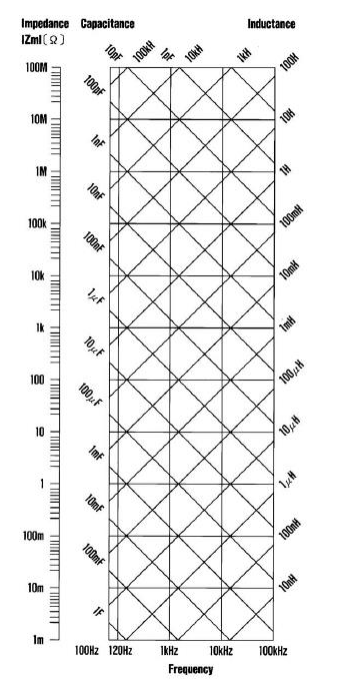
\includegraphics[height=20cm, width=12cm]{media/diagramma_conversione_Cp.png}
    \caption{Diagramma di conversione}
    \label{fig:diag_conv_Cp}
\end{figure}
\FloatBarrier
\clearpage

Consultando le tabelle di incertezza fornite dal costruttore avremo:

\begin{table}[H]
\centering
\resizebox{\textwidth}{!}{%
\begin{tabular}{|c|c|c|c|c|c|c|c|}
\hline
\textbf{A}      & \textbf{B}      & \textbf{C} & \textbf{D [$\bm{\Omega}$]} & \textbf{E [$\bm{\Omega}$]} & \textbf{Zs [$\bm{\Omega}$]} & \textbf{Zx} {\tiny(Cp convertito)}  \textbf{[$\bm{\Omega}$]} & \textbf{Uz (Ae)} \\ \hline
0,0048  & 0,00055 & 1 & 0,01      & 280.000.000,00  & 100000          & 228054,8849     & 0,0069  \\ \hline
0,0048  & 0,00055 & 1 & 0,01      & 280.000.000,00  & 100000          & 192858,9781     & 0,0065  \\ \hline
0,0011  & 0,0002 & 1 & 0,0165    & 28.000.000,00  & 10000          & 22880,2391     & 0,0024  \\ \hline
0,0016  & 0,0002 & 1 & 0,075     & 2.800.000,00  & 1000          & 2311,4843     & 0,0029  \\ \hline
0,0112 & 0,0011 & 1 & 0,75      & 280.000,00  & 100          & 237,4632     & 0,0178  \\ \hline
\end{tabular}%
}
\caption{Tabella di incertezza fornita dal costruttore, con Uz l'incertezza}
\label{tab:lcr_c_sheet}
\end{table}
\FloatBarrier

L’incertezza della resistenza parallelo, invece, si calcola come:

\begin{equation}
        U_{R_P} = \pm \frac{Rp_X \times D_e}{D_X \mp D_e}  \\
\end{equation}

dove $Rp_X$ indica il valore misurato della resistenza parallelo in $\Omega$, $D_e$ è l’incertezza di 
$D$, mentre $D_X$ è il valore misurato di $D$.

L’incertezza dell’angolo di perdita, $D_e$, si calcola come:

\begin{equation}
    D_e = \pm \frac{A_e}{100}
\end{equation}

Se il valore misurato di $D$ risulta ad essere maggiore di 0,1 , allora bisogna 
moltiplicare $D_e$ per $(1+D_X)$. L’incertezza sulla resistenza parallelo si applica solo 
quando il valore misurato di $D$ è minore di 0,1.

Nella seguente tabella è riassunto quanto detto precedentemente:

\begin{table}[H]
\centering
\resizebox{\textwidth}{!}{%
\begin{tabular}{|c|c|c|c|}
\hline
\textbf{ Rp$\bm{_X}$ [$\bm{\Omega}$]} & \textbf{De}  & \textbf{Dx}  & \textbf{U(Rp)} \\ \hline
1,27E+08                    & 0,000069    & 0,0018     & 5.056.466,99    \\ \hline
1,33E+08                    & 0,000065    & 0,0017    & 5.317.770,16      \\ \hline
5,42E+06                    & 0,000024    & 0,0039     & 33.193,91      \\ \hline
2,60E+05                    & 0,000029    & 0,0095     & 800,46      \\ \hline
1,87E+04                    & 0,000178    & 0,0147     & 229,45      \\ \hline
\end{tabular}%
}
\caption{LCR, misura della resistenza}
\label{tab:lcr_c_RPx}
\end{table}
\FloatBarrier
\clearpage


    
    %\hypersetup{hidelinks}
    %\input{./chapters/mult.tex}
    
    %\hypersetup{hidelinks}
    %\input{./chapters/lcr.tex}
    
    % Chapter 3
    \hypersetup{hidelinks}
    \chapter{Compensazione in frequenza di una sonda  e Caratterizzazione di un filtro RC}
\label{chap:seconda_prova}

\section*{Obiettivo}
\label{sec:ob_second}
L'obiettivo della seconda esperienza di laboratorio è quello di effettuare la compensazione in frequenza di una sonda e poi di ricavare i diagrammi di Bode di un filtro passabasso passivo RC, i valori di \emph{attenuazione} e \emph{sfasamento} con le relative \emph{incertezze} mediante valutazioni di tipo B.

\section{Compensazione in frequenza di una sonda}
Le sonde costituiscono un componente fondamentale per poter prelevare un segnale da osservare e da trasferire poi allo strumento.

\begin{figure}[h]
    \centering
    \includegraphics[height=7cm]{sonda.png}
    \caption{Sonda}
    \label{fig:sonda}
\end{figure}

La sonda può essere schematizzata in maniera semplificata come un parallelo di una resistenza e una capacità variabile. L'oscilloscopio d'altra parte ha una certa capacità intrinseca in parallelo ad una resistenza di ingresso. Tale capacità in regime AC può essere un problema, in quanto all'aumentare della frequenza inizia ad agire come un filtro passa-basso.

Per questo motivo è necessario effettuare la \textbf{compensazione in frequenza della sonda}, cioè impostare il valore della capacità variabile della sonda per andare a compensare gli effetti della capacità di ingresso dell'oscilloscopio, quindi da rendere il sistema sonda+oscilloscopio indipendente dalla frequenza.

\subsection*{}
Per poter effettuare la compensazione, abbiamo collegato il connettore BNC della sonda al canale 1 dell'oscilloscopio. Abbiamo poi sollevato il cappuccio della sonda e l'abbiamo collegata all'occhiello presente nella parte inferiore del dispositivo, che risulta essere la sorgente di onda quadra di ampiezza 5V e frequenza 1.2KHz generata dall'oscilloscopio stesso.

Abbiamo poi premuto il tasto \textbf{Autoscale} per visualizzare il segnale sullo schermo.

Poiché la sonda fornisce un'attenuazione pari a 10, premendo sul tasto 1 della sezione verticale, è possibile impostare il valore di \emph{Probe} su 10, mediante il tasto presente sotto lo schermo, in modo che la lettura sia riferita all'attenuazione implicita della sonda.

Fatto ciò abbiamo sistemato i valori di $K_v$ e $K_t$ per visualizzare circa 2 periodi e in modo ottimale sullo schermo l'onda quadra.

Abbiamo infine utilizzato un cacciavite in prossimità del corpo della sonda, per regolare la capacità variabile, finché il segnale visualizzato non è apparso quanto più rettangolare possibile rispetto alla condizione iniziale in cui erano presenti delle sovra-elongazioni dovute alla sovracompensazione.


\clearpage
\section{Caratterizzazione di un Filtro RC} \label{sec:filtroRC}
Nel seguente paragrafo verrà descritto in breve il filtro RC e le sue caratteristiche. Seguirà una presentazione della strumentazione utilizzata, la descrizione della configurazione dei dispositivi e la procedura di misura.

\subsection{Filtro RC}
Il filtro RC è un sistema che effettua sul suo segnale di ingresso una funzione di attenuazione in quanto filtro passivo, cioè composto da componenti passivi quali un condensatore e un resistore in serie.

\begin{figure}[h]
    \centering
    \includegraphics[height=5cm]{filtroRC.png}
    \caption{Filtro RC}
    \label{fig:filtroRC}
\end{figure}
\FloatBarrier

Esso è un filtro passa basso che cioè permette il passaggio delle frequenze al di sotto di una \textbf{frequenza di taglio} e attenua invece quelle alte. In particolare, l'attenuazione $A$ del filtro RC è definita come:

\[A=\frac{V_o}{V_i}=\frac{1}{1+j\omega RC}\]

La frequenza di taglio del filtro è definita come la frequenza alla quale la potenza del segnale in uscita dal filtro è pari alla metà della potenza del segnale in ingresso ad esso. Oppure è definita come la frequenza alla quale la tensione disponibile in uscita è $1/\sqrt{2}$ la tensione di ingresso disponibile in banda passante.

La frequenza di taglio \emph{teorica} si calcola uguagliando il modulo dell'attenuazione $A$ al valore $1/\sqrt{2}$

\[\frac{1}{\sqrt{1+(\omega RC)^2}} = \frac{1}{\sqrt{2}}\]
\[1+(\omega RC)^2 = 2\] 
\[(\omega RC)^2 = 1\]
\[\omega ^2 = \frac{1}{(RC)^2}\]
Ricordando che $\omega = 2\pi f$, si ha che la frequenza di taglio è pari a 
\[f=\frac{1}{2\pi RC}\]

\subsection{Strumentazione utilizzata}
\subsection*{PCB}
Il PCB (Printed Circuit Board) è una scheda elettronica fornita durante l'esercitazione, sulla quale, mediante l'utilizzo di jumper come nella configurazione in Figura \ref{fig:pcb_rc}, è stato realizzato un filtro RC, i cui valori di resistenza e capacità sono rispettivamente 10k$\Omega$ e 47nF.

\begin{figure}[h]
    \centering
    \includegraphics[width=0.9\linewidth]{PCB.png} 
    \caption{PCB}
    \label{fig:pcb}
\end{figure}

\begin{figure}[h]
    \centering
    \includegraphics[width=0.9\linewidth, height=14cm]{PCB_RC.png}
    \caption{Configurazione di filtro RC del PCB}
    \label{fig:pcb_rc}
\end{figure}
\FloatBarrier

\clearpage
\subsection*{Oscilloscopio Agilent Hp 54600B}
\begin{figure}[h]
    \centering
    \includegraphics[width=0.8\linewidth, height=7cm]{oscilloscopio.png}
    \caption{Oscilloscopio Agilent HP 54600B}
    \label{fig:enter-label}
\end{figure}
\FloatBarrier

\subsection*{Generatore di funzioni Agilent 33120B}
\begin{figure}[h]
    \centering
    \includegraphics[width=\linewidth, height=6cm]{gen_fun.png}
    \caption{Generatore di funzioni Agilent 33120B}
    \label{fig:gen_fun}
\end{figure}
\FloatBarrier
\clearpage

\subsection*{Cavi di connessione (BNC-BNC)}
\begin{figure}[h]
    \centering
    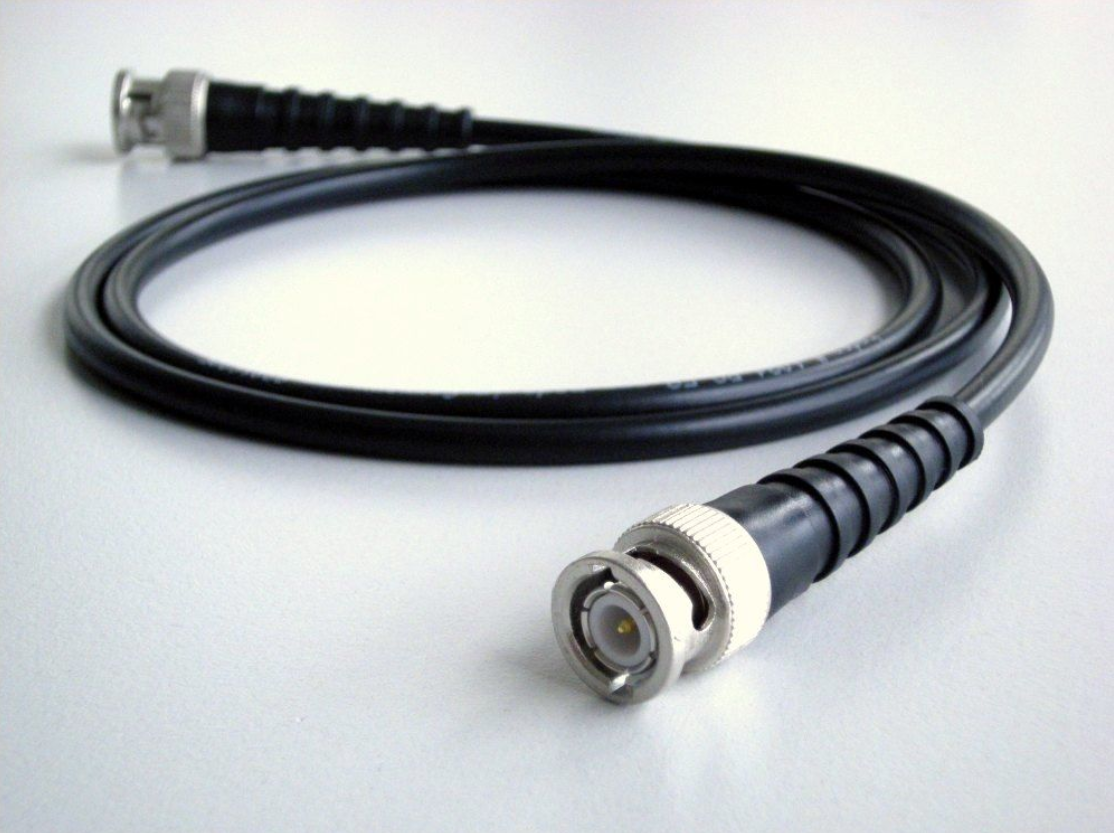
\includegraphics[width=0.75\linewidth]{media/cavoBNC.png}
    \caption{Cavo di connessione BNC-BNC}
    \label{fig:enter-label}
\end{figure}
\FloatBarrier
\clearpage

\subsection{Configurazione della strumentazione per la misurazione}

Prima di iniziare ad effettuare le misurazioni del caso, abbiamo configurato tutte le strumentazioni a disposizione. Abbiamo dunque:

\begin{itemize}
    \item Collegato i cavi di connessione secondo la seguente configurazione:
    \begin{itemize}
        \item Uscita del generatore di funzioni all'ingresso (BNC INPUT) del filtro RC
        \item Ingresso del filtro RC (BNC OUTPUT 1) al canale 1 dell'oscilloscopio
        \item Uscita del filtro RC (BNC OUTPUT 2) al canale 2 dell'oscilloscopio
    \end{itemize}
    \begin{figure}[h]
        \centering
        \includegraphics{PCB_bnc.png}
        \caption{Ingressi/Uscite del filtro RC}
        \label{fig:pcb_bnc}
    \end{figure}
    \begin{figure}[h]
        \centering
        \includegraphics[width=0.6\linewidth]{conf_bnc.png}
        \caption{Configurazione dei cavi di connessione}
        \label{fig:conf_bnc}
    \end{figure}
    \FloatBarrier

    \item Avviato il generatore di funzioni impostando una frequenza iniziale di 100kHz mediante il tasto \emph{Freq} e successivamente impostato una forma d'onda sinusoidale di ampiezza pari a 5 V mediante il tasto \emph{Ampl}.
    
    \'E importante osservare che l'ampiezza visualizzata sull'oscilloscopio è diversa da quella impostata sul generatore di funzioni a causa del disadattamento di impedenza tra l'oscilloscopio ed il generatore di funzioni. In particolare, in corrispondenza della tensione picco-picco di 5 V impostata per l'ingresso del filtro, verrà visualizzata una tensione picco-picco di 10 V sul display dell'oscilloscopio.
    \item Avviato l'oscilloscopio su cui visualizzare il segnale d'ingresso del filtro $V_i$ sul canale 1, e il segnale di uscita del filtro $V_o$ sul canale 2.
    Poiché abbiamo utilizzato cavi BNC-BNC e non sonde, abbiamo impostato il valore di \emph{Probe} a 1 mediante l'apposito pulsante posto sotto lo schermo.
    Per migliorare la visualizzazione di entrambi i segnali, abbiamo premuto il pulsante \emph{Auto-Scale}, che permette all'oscilloscopio di visualizzare entrambi i segnali, uno per ognuno della due metà dello schermo.
    
    Ai fini delle misurazioni da effettuare, abbiamo impostato entrambe le forme d'onda sulla linea di 0 V secondo la seguente procedura per entrambi i canali:
    \begin{enumerate}
        \item Selezione del singolo canale dal rispettivo pulsante della sezione verticale
        \item Impostazione del \emph{Coupling} su Ground mediante il secondo pulsante posizionato sotto lo schermo
        \item Utilizzo della manopola presente sotto la sezione Measure per spostare il riferimento del segnale sulla linea di 0 V
        \item Impostazione del \emph{Coupling} su AC mediante il secondo pulsante posizionato sotto lo schermo  
    \end{enumerate}
\end{itemize}

\clearpage


\subsection{Misurazioni}

\subsubsection{Calcolo della frequenza di taglio sperimentale}

Come definito nel paragrafo introduttivo sul filtro RC (\ref{sec:filtroRC}), la frequenza di taglio teorica è pari a
\[f=\frac{1}{2\pi RC}= \frac{1}{2\pi \cdot10^4 \cdot 47 \cdot10^{-9}} = 338,627 Hz\]
Questa tuttavia non sarà mai pari a quella effettiva, pertanto abbiamo ricavato sperimentalmente la frequenza di taglio effettiva. Poiché il segnale in ingresso era pari a 5 V, visualizzati 10V sull'oscilloscopio, la frequenza di taglio è quella frequenza in corrispondenza della quale l'uscita $V_{o}$ del filtro è pari a 
\[\frac{10}{\sqrt{2}} = 7,07 V\]

Abbiamo allora premuto prima sul pulsante \emph{Cursors}, selezionato il cursore $V_1$ posizionandolo per mezzo della manopola ad un valore di 3,5 V, 
e il cursore $V_2$ posizionandolo ad un valore di -3,5 V. In questo modo la distanza tra i due cursori era pari a 7 V.

Andando quindi ad operare sul generatore di funzioni, abbiamo modificato la frequenza del segnale in ingresso al filtro finché il segnale di uscita (canale 2) non appariva esattamente tangente ai due cursori precedentemente posizionati.
La frequenza per cui tale condizione è soddisfatta corrisponde alla frequenza di taglio reale del filtro che è pari a 
\[f_{sperimentale} = 338,63Hz\]

In base al datasheet del generatore di funzioni, il valore dell'incertezza relativa di caso peggiore per misure di frequenza è di 20 ppm (parti per milione), cioè 
\[U_{r,f} = 20 ppm\]
L'incertezza assoluta di caso peggiore sarà pari a
\[U_f = 338 Hz\cdot U_{r,f} = 338,63Hz \cdot 20 \cdot 10^{-6} = 6,773\cdot10^{-3}Hz\]


\clearpage
\subsubsection{Misure di tensione picco-picco e $\Delta t$}

Per riuscire a ricavare i valori necessari a graficare i diagrammi di Bode dell'attenuazione A del filtro RC, è stato necessario ripetere la stessa procedura di misura, lasciando invariate le condizioni operative, per un totale di 17 diversi valori di frequenza.

Per ogni misurazione abbiamo quindi eseguito i seguenti passi:
\begin{enumerate}
    \item Impostato il valore della frequenza del segnale di ingresso del filtro  sul generatore di funzioni, premendo prima il pulsante \emph{Freq} e poi impostando la frequenza desiderata \footnote{Per misurazioni effettuate a frequenze molto basse, intorno ai pochi Hz, per visualizzare correttamente il segnale è stato utile premere il tasto \textbf{Mode} della sezione Trigger, e impostare tramite il tasto presente sotto lo schermo, la modalità \textbf{Normal}.} \footnote{Per misurazioni effettuate a frequenze molto elevate, per ridurre il rumore sul segnale è stato utile premere sul tasto \textbf{Display}, posto sopra la sezione verticale, per impostare tramite il pulsante apposito sotto lo schermo la modalità \textbf{Average}.} .
    \item Regolato i valori di $K_{V_i}$ e $K_{V_o}$ mediante le manopole poste nella parte superiore della sezione verticale, in modo da coprire quanto più possibile lo schermo senza tagliare la forma d'onda. In questo modo le misure eseguite sono più accurate e viene ridotta l'incertezza di misura.
    \item Regolato il valore di $K_t$ mediante l'apposita manopola posta nella sezione orizzontale per la visualizzazione di almeno un periodo dei segnali.
    \item Premuto il pulsante \emph{Voltage}, situato nella sezione \emph{Measure} e selezionato per ognuno dei due segnali il tipo di misura, cioè tensione picco-picco $V_{p-p}$, mediante gli appositi pulsanti posizionati sotto lo schermo.
    In questo modo i valori di tensione picco-picco di entrambi i segnali vengono automaticamente calcolati dall'oscilloscopio e visualizzati nella parte inferiore dello schermo.
    \item Sistemato il valore di $K_t$ per visualizzare meglio il punto in cui ciascun segnale tagliava l'asse delle ascisse, premuto il pulsante \emph{Cursors} e selezionato i cursori verticali $t_1$ e $t_2$, dagli appositi pulsanti posti sotto lo schermo. Ciascun cursore , mediante la manopola presente sotto la sezione \emph{Measure}, è stato poi collocato in corrispondenza dei punti in cui il corrispondente segnale passava per lo zero. Il valore $\Delta t$  calcolato dall'oscilloscopio è poi visualizzato nella parte inferiore dello schermo. 
    
\end{enumerate}




\clearpage

\subsection{Calcolo delle incertezze}
In questo paragrafo si effettuerà sulle misure ottenute la valutazione dell'incertezza di \textbf{tipo B}, basata sull'utilizzo di informazioni note a priori quali le specifiche metrologiche degli strumenti adoperati.

\subsubsection{Misure Dirette}

Le misure dirette effettuate durante l'esperienza di laboratorio sono le seguenti:
\begin{itemize}
    \item \textbf{tensione picco-picco V}
    \item \textbf{distanza temporale $\Delta t$}  fra i segnali sinusoidali $V_i$ e $V_o$
    \item \textbf{frequenza f} dei segnali $V_i$ e $V_o$ 
\end{itemize}


\subsubsection*{Incertezza associata alle misure di tensione picco-picco V}

Dalle specifiche metrologiche di ampiezza dell'oscilloscopio, poiché abbiamo utilizzato i due cursori orizzontali per le misure, consideriamo la \textbf{Dual cursor accuracy}, pari a 
\[vertical \ accuracy \pm 0.4\% \ of full scale\]

dove \textbf{vertical accuracy} per l'oscilloscopio Agilent HP 54600B è pari a 1.9\%, mentre \textbf{full scale} è il fondo scala del dispositivo ed è pari a $y_{FS} = 8 \cdot k_v$, dove 8 sono le divisioni verticali e $k_v$ è la \emph{vertical sensitivity} espressa in V/div.

La \emph{Dual cursor accuracy} sopra riportata deriva dalla formula generale dell'incertezza per una differenza 
\[U(V_1 - V_2) = U_G|V_1 - V_2| + 2U_{inl} + 2U{q}\]

Nel nostro caso, l'incertezza di non linearità integrale $U_{inl}$, è stata conglobata nel termine 1.9\% insieme a $U_G$ incertezza di guadagno. L'incertezza di quantizzazione $2U_q$ è invece pari al termine $\pm 0.4\% \cdot y_{FS}$. L'incertezza di offset $U_O$ non è presente poiché nel caso di differenze di misure l'errore di offset si compensa.

Indicato quindi con $V$ il valore di tensione picco-picco letto, l'\textbf{incertezza di caso peggiore} associata a $V$ è data dalla seguente formula:

\[U_V = \frac{1.9}{100} \cdot |V| + \frac{0.4}{100} \cdot 8 \cdot k_v\]

Da questa formula è possibile poi ricavare l'\textbf{incertezza relativa di caso peggiore}:
\[U_{r,V} = \frac{U_V}{V}\]

Seguono due tabelle contenenti per ogni valore di frequenza: il valore di tensione letto, la vertical sensitivity all'atto della lettura, l'incertezza assoluta di caso peggiore e l'incertezza relativa di caso peggiore.

\begin{table}[!ht]
    \centering
    \begin{tabular}{|c|c|c|c|c|}
    \hline

        \textbf{f [Hz]} & \textbf{$\bm{V_{i}}$ [V]} & \textbf{$\bm{K_{V_i}}$ [V/div]} & \textbf{U($\bm{V_{i}}$)} & \textbf{$\bm{U_{r}}$($\bm{V_{i}}$)} \\ \hline

        1 & 1 & 3,938 & 1 & 0,11 & 0,027 \\ \hline
        2 & 2 & 6,468 & 1 & 0,15 & 0,024 \\ \hline
        3 & 3 & 7,875 & 2 & 0,21 & 0,027 \\ \hline
        4 & 6 & 9,375 & 2 & 0,24 & 0,026 \\ \hline
        5 & 10 & 9,75 & 2 & 0,25 & 0,026 \\ \hline
        6 & 18 & 10 & 2 & 0,25 & 0,025 \\ \hline
        7 & 32 & 10,12 & 2 & 0,26 & 0,025 \\ \hline
        8 & 56 & 10,25 & 2 & 0,26 & 0,025 \\ \hline
        9 & 100 & 10,12 & 2 & 0,26 & 0,025 \\ \hline
        10 & 180 & 10 & 2 & 0,25 & 0,025 \\ \hline
        11 & 320 & 9,875 & 2 & 0,25 & 0,025 \\ \hline
        12 & 560 & 9,75 & 2 & 0,25 & 0,026 \\ \hline
        13 & 1000 & 8,875 & 2 & 0,23 & 0,026 \\ \hline
        14 & 1800 & 9,625 & 2 & 0,25 & 0,026 \\ \hline
        15 & 3200 & 9,875 & 2 & 0,25 & 0,025 \\ \hline
        16 & 5600 & 9,875 & 2 & 0,25 & 0,025 \\ \hline
        17 & 10000 & 9,875 & 2 & 0,25 & 0,025 \\ \hline
    \end{tabular}
\end{table}

\begin{table}[!ht]
    \centering
    \begin{tabular}{|c|c|c|c|c|}
    \hline

        \textbf{f [Hz]} & \textbf{$\bm{V_{o}}$ [V]} & \textbf{$\bm{K_{V_o}}$ [V/div]} & \textbf{U($\bm{V_{o}}$)} & \textbf{$\bm{U_r}$($\bm{V_{o}}$)} \\ \hline

        1 & 4 & 1 & 0,11 & 0,027 \\ \hline
        2 & 6,531 & 1 & 0,16 & 0,024 \\ \hline
        3 & 7,875 & 2 & 0,21 & 0,027 \\ \hline
        6 & 9,25 & 2 & 0,24 & 0,026 \\ \hline
        10 & 9,635 & 2 & 0,25 & 0,026 \\ \hline
        18 & 9,875 & 2 & 0,25 & 0,025 \\ \hline
        32 & 9,938 & 2 & 0,25 & 0,025 \\ \hline
        56 & 10 & 2 & 0,25 & 0,025 \\ \hline
        100 & 9,625 & 2 & 0,25 & 0,026 \\ \hline
        180 & 8,75 & 2 & 0,23 & 0,026 \\ \hline
        320 & 7,188 & 2 & 0,20 & 0,028 \\ \hline
        560 & 5,125 & 2 & 0,16 & 0,031 \\ \hline
        1000 & 2,859 & 0,50 & 0,070 & 0,025 \\ \hline
        1800 & 1,797 & 0,50 & 0,050 & 0,028 \\ \hline
        3200 & 1,05 & 0,20 & 0,026 & 0,025 \\ \hline
        5600 & 0,606 & 0,10 & 0,015 & 0,024 \\ \hline
        10000 & 0,342 & 0,05 & 0,0081 & 0,024 \\ \hline
    \end{tabular}
\end{table}

\FloatBarrier
\clearpage


\subsubsection*{Incertezza temporale associata alle misure di distanza temporale $\Delta t$}

Le specifiche metrologiche della base dei tempi dell'oscilloscopio forniscono la seguente espressione per la \textbf{Delta t accuracy}:

\[\pm0.01\% \pm0.2\% \ of full scale \pm 200 \ ps\]

Possiamo dare un'interpretazione dell'espressione a partire dalla formula dell'incertezza sulla differenza di misure di tempo:
\[U(T_1 - T_2) = U_S |T_1 - T_2| + 2U_{tbd} + 2U_{T_c}\]

$U_S$ incertezza sulla velocità di sweep, equivale al coefficiente $\pm0.01\%$.
$2U_{tbd}$ incertezza di distorsione della base dei tempi è pari al valore $\pm200 \ ps$.
$2U_{T_c}$ incertezza di risoluzione, equivale al termine $\pm0.2\% \ of full scale$, dove full scale è il valore di fondoscala pari a $\tau _{FS}  = 10 \cdot k_t$.
Infine, poiché si parla di differenze di misure, l'incertezza di ritardo del trigger $U_D$ è trascurabile.

Indicato con $\Delta t$ il valore di distanza temporale tra i segnali $V_i$ e $V_o$, l'\textbf{incertezza assoluta di caso peggiore} associata a $\Delta t$ è data dalla seguente formula:

\[U_{\Delta t} = \frac{0.01}{100} \cdot |\Delta t| + \frac{0.2}{100} \cdot  10 \cdot k_t + 200 \ ps  \]

Da questa formula è possibile poi ricavare l'\textbf{incertezza relativa di caso peggiore}:
\[U_{r,\Delta t} = \frac{U_{\Delta t}}{\Delta t}\]

Segue per ogni valore di frequenza: il valore di $\Delta t$ letto, il valore di $k_t$, l'incertezza (assoluta e relativa) di caso peggiore

\begin{table}[!ht]
    \centering
    \begin{tabular}{|c|c|c|c|c|}
    \hline

        \textbf{f [Hz]} & \textbf{$\bm{\Delta t}$ [µs]} & \textbf{$\bm{K_t}$ [µs/div]} & \textbf{U($\bm{\Delta t}$)} & \textbf{$\bm{U_r(\Delta t)}$} \\ \hline

        1 & 3200 & 500,00 & 0,000010 & 0,0032 \\ \hline
        2 & 2140 & 500,00 & 0,000010 & 0,0048 \\ \hline
        3 & 1550 & 200,00 & 0,0000042 & 0,0027 \\ \hline
        6 & 684 & 100,00 & 0,0000021 & 0,0030 \\ \hline
        10 & 592 & 100,00 & 0,0000021 & 0,0035 \\ \hline
        18 & 500 & 100,00 & 0,0000021 & 0,0041 \\ \hline
        32 & 480 & 100,00 & 0,0000020 & 0,0043 \\ \hline
        56 & 464 & 100,00 & 0,0000020 & 0,0044 \\ \hline
        100 & 448 & 200,00 & 0,0000040 & 0,0090 \\ \hline
        180 & 424 & 100,00 & 0,0000020 & 0,0048 \\ \hline
        320 & 370 & 50,00 & 0,0000010 & 0,0028 \\ \hline
        560 & 276 & 50,00 & 0,0000010 & 0,0037 \\ \hline
        1000 & 203 & 50,00 & 0,0000010 & 0,0050 \\ \hline
        1800 & 128 & 20,00 & 0,00000041 & 0,0032 \\ \hline
        3200 & 77 & 10,00 & 0,00000021 & 0,0027 \\ \hline
        5600 & 43 & 10,00 & 0,00000020 & 0,0048 \\ \hline
        10000 & 24 & 5,00 & 0,00000010 & 0,0042 \\ \hline
    \end{tabular}
\end{table}
\FloatBarrier
\clearpage


\subsubsection*{Incertezza associata alle misure di frequenza f}

Le specifiche metrologiche del generatore di funzioni, forniscono il valore dell'\textbf{incertezza relativa di caso peggiore} per le misure di frequenza, pari a :

\[U_{r,f} = 20 \ ppm\]

Da questa espressione è possibile ricavare l'\textbf{incertezza assoluta di caso peggiore}:

\[U_f = f \cdot U_{r,f}\]
Di seguito i valori di incertezza per ogni valore di frequenza 

\begin{table}[!ht]
    \centering
    \begin{tabular}{|c|c|c|}
    \hline

        \textbf{f [Hz]} & \textbf{U(f)} & $\bm{U_r(f)}$ [ppm] \\ \hline

        1 & 0,000020 & 20 \\ \hline
        2 & 0,000040 & 20 \\ \hline
        3 & 0,000060 & 20 \\ \hline
        6 & 0,00012 & 20 \\ \hline
        10 & 0,00020 & 20 \\ \hline
        18 & 0,00036 & 20 \\ \hline
        32 & 0,00064 & 20 \\ \hline
        56 & 0,0011 & 20 \\ \hline
        100 & 0,0020 & 20 \\ \hline
        180 & 0,0036 & 20 \\ \hline
        320 & 0,0064 & 20 \\ \hline
        560 & 0,011 & 20 \\ \hline
        1000 & 0,020 & 20 \\ \hline
        1800 & 0,036 & 20 \\ \hline
        3200 & 0,064 & 20 \\ \hline
        5600 & 0,11 & 20 \\ \hline
        10000 & 0,20 & 20 \\ \hline
    \end{tabular}
\end{table}

\FloatBarrier
\clearpage


\subsubsection{Misure Indirette}

Le misure indirette eseguite sono:
\begin{itemize}
    \item \textbf{Attenuazione $A$}
    \item \textbf{Sfasamento $\Delta \varphi$}
\end{itemize}


\subsubsection*{Incertezza associata alle misure di attenuazione $A$}

Ricordiamo che l'attenuazione $A$ del filtro RC è definita come
\[A = \frac{V_o}{V_i}\]
cioè è data dal rapporto di due misure dirette. Pertanto, per poter stimare l'incertezza di $A$, occorre ricorrere alla \textit{formula di propagazione delle incertezze di caso peggiore}:
\[U = \sum_{n=1}^{N} \left|\frac{\partial f}{\partial y_i}\right| \cdot U_i\]

Dall'applicazione di tale formula, nel caso di rapporto tra misure, si ha che l'\textbf{incertezza relativa} è data dalla \textbf{somma delle incertezze relative} delle singole misure dirette. Pertanto nel nostro caso essa è pari a:

\[U_{r,A} = U_{r,V_o} + U_{r,V_i}\]

da cui si ha\textbf{ l'incertezza assoluta di caso peggiore}:

\[U_A = A \cdot U_{r,A}\]

Solitamente i valori di attenuazione $A$ vengono riportati in dB(decibel) secondo la formula:

\[A_{dB} = 20\cdot \log_{10} A\]

Applicando la formula di propagazione dellle incertezze si ottiene l'espressione per l'\textbf{incertezza assoluta di caso peggiore} $U_{A_{db}}$:

\[U_{A_{db}} = \frac{20}{\ln 10} \cdot U_{r,A}\]

Segue la tabella riportante per ogni valore di frequenza: il valore calcolato di $A$ con relativa incertezza (assoluta e relativa) di caso peggiore e il valore in dB di $A$ con relativa incertezza (assoluta e relativa) di caso peggiore.

\begin{table}[!ht]
    \centering
    \begin{tabular}{|c|c|c|c|c|c|c|}
    \hline

        \textbf{FREQ [Hz]} & \textbf{A} & \textbf{U(A)} & $\bm{U_r(A)}$ & $\bm{A_{dB}}$ & \textbf{U($\bm{A_{dB}}$)} & $\bm{U_r(A_{dB})}$ \\ \hline

        1 & 1,016 & 0,055 & 0,054 & 0,1357 & 0,47 & 3,46 \\ \hline
        2 & 1,010 & 0,048 & 0,048 & 0,08419 & 0,42 & 4,94 \\ \hline
        3 & 1,000 & 0,054 & 0,054 & 0,0000 & 0,47 & - \\ \hline
        6 & 0,9867 & 0,051 & 0,052 & -0,1166 & 0,45 & -3,85 \\ \hline
        10 & 0,9882 & 0,051 & 0,051 & -0,1031 & 0,44 & -4,32 \\ \hline
        18 & 0,9875 & 0,050 & 0,051 & -0,1093 & 0,44 & -4,04 \\ \hline
        32 & 0,9820 & 0,050 & 0,051 & -0,1576 & 0,44 & -2,80 \\ \hline
        56 & 0,9756 & 0,049 & 0,051 & -0,2145 & 0,44 & -2,05 \\ \hline
        100 & 0,9511 & 0,048 & 0,051 & -0,4356 & 0,44 & -1,02 \\ \hline
        180 & 0,8750 & 0,045 & 0,052 & -1,160 & 0,45 & -0,39 \\ \hline
        320 & 0,7279 & 0,039 & 0,053 & -2,759 & 0,46 & -0,17 \\ \hline
        560 & 0,5256 & 0,030 & 0,057 & -5,586 & 0,50 & -0,089 \\ \hline
        1000 & 0,3221 & 0,016 & 0,051 & -9,839 & 0,44 & -0,045 \\ \hline
        1800 & 0,1867 & 0,010 & 0,054 & -14,58 & 0,47 & -0,032 \\ \hline
        3200 & 0,1063 & 0,0054 & 0,051 & -19,47 & 0,44 & -0,023 \\ \hline
        5600 & 0,06139 & 0,0031 & 0,050 & -24,24 & 0,43 & -0,018 \\ \hline
        10000 & 0,03465 & 0,0017 & 0,049 & -29,21 & 0,43 & -0,015 \\ \hline
    \end{tabular}
\end{table}

\FloatBarrier
\clearpage


\subsubsection*{Incertezza associata alle misure di sfasamento $\Delta \varphi$}


Come l'attenuazione, anche lo sfasamento $\Delta \varphi$ è una misura indiretta, ottenuta dalla formula
\[\Delta \varphi =  -2\pi \cdot f \cdot \Delta t  \]

Pertanto è necessario ricorrere alla legge di propagazione delle incertezze, osservando che nel caso di prodotto di misure dirette, le \textbf{incertezze relative si sommano}, ovvero:
\[U_{r,\Delta \varphi} = U_{r,f} + U_{r,\Delta t}\]

Per le misure di sfasamento, abbiamo provveduto a calcolare anche l'incertezza standard. A partire dalla formula per il calcolo dell'incertezza standard, osservando che $f$ e $\Delta t$ sono \emph{scorrelate}, si ha la seguente espressione per \textbf{l'incertezza standard}:
\[u_{\Delta \varphi} = \Delta\varphi \cdot \sqrt{\frac{U_{r,f}^2}{3}+ \frac{U_{r,\Delta t}^2}{3}}\]

da cui\textbf{ l'incertezza standard relativa}:
\[u_{r,\Delta \varphi} = \sqrt{\frac{U_{r,f}^2}{3}+ \frac{U_{r,\Delta t}^2}{3}}\]

Segue una tabella dove per i diversi valori di frequenza sono indicati i valori di $\Delta\varphi$, di incertezza (assoluta e relativa) di caso peggiore e di incertezza standard (assoluta e relativa).

\begin{table}[!ht]
    \centering
    \begin{tabular}{|c|c|c|c|c|c|}
    \hline

        \textbf{f [Hz]} & $\bm{\Delta\varphi}$ \textbf{[rad]} & $\bm{U(\Delta\varphi)}$ & $\bm{U_r(\Delta\varphi)}$ & $\bm{u(\Delta\varphi)}$ & $\bm{u_r(\Delta\varphi)}$ \\ \hline

        1 & -0,02011 & 0,000065 & 0,0032 & 0,000037 & 0,0019 \\ \hline
        2 & -0,02689 & 0,00013 & 0,0048 & 0,000074 & 0,0028 \\ \hline
        3 & -0,02922 & 0,000079 & 0,0027 & 0,000045 & 0,0015 \\ \hline
        6 & -0,02579 & 0,000079 & 0,0030 & 0,000045 & 0,0017 \\ \hline
        10 & -0,03720 & 0,00013 & 0,0035 & 0,000075 & 0,0020 \\ \hline
        18 & -0,05655 & 0,00023 & 0,0041 & 0,00013 & 0,0024 \\ \hline
        32 & -0,09651 & 0,00041 & 0,0043 & 0,00024 & 0,0025 \\ \hline
        56 & -0,1633 & 0,00072 & 0,0044 & 0,00042 & 0,0025 \\ \hline
        100 & -0,2815 & 0,0025 & 0,0090 & 0,0015 & 0,0052 \\ \hline
        180 & -0,4795 & 0,0023 & 0,0048 & 0,0013 & 0,0028 \\ \hline
        320 & -0,7439 & 0,0021 & 0,0028 & 0,0012 & 0,0016 \\ \hline
        560 & -0,9711 & 0,0036 & 0,0037 & 0,0021 & 0,0022 \\ \hline
        1000 & -1,275 & 0,0064 & 0,0050 & 0,0037 & 0,0029 \\ \hline
        1800 & -1,443 & 0,0047 & 0,0033 & 0,0027 & 0,0019 \\ \hline
        3200 & -1,556 & 0,0042 & 0,0027 & 0,0024 & 0,0016 \\ \hline
        5600 & -1,506 & 0,0072 & 0,0048 & 0,0042 & 0,0028 \\ \hline
        10000 & -1,533 & 0,0065 & 0,0042 & 0,0037 & 0,0024 \\ \hline
    \end{tabular}
\end{table}

\subsubsection*{Seguono i diagrammi di Bode di modulo e fase }


% Diagramma di Bode del modulo
\begin{figure}[h]
    \centering
    \resizebox{0.80\textwidth}{!}{%
    \begin{tikzpicture}
        \begin{axis}
            [xlabel={Decadi di frequenza}, ylabel={A\textsubscript{dB}}, 
            xtick={0,1,2,3,4}, xticklabels={$10^0$, $10^1$, $10^2$, $10^3$, $10^4$}]
            \addplot[red, mark=*, only marks] 
            table[x=x, y=y,y error=error, col sep=comma] {media/bode/bode_adb_logf_2prova.txt};
        \end{axis}
    \end{tikzpicture}
    }%
    \caption{Diagramma di Bode del modulo}
    \label{fig:amplitude}
\end{figure}
% Diagramma di Bode della fase
\begin{figure}[h]
    \centering
    \resizebox{0.80\textwidth}{!}{%
    \begin{tikzpicture}
        \begin{axis}
            [xlabel={Decadi di frequenza}, ylabel={$\Delta\varphi$}, 
            xtick={0,1,2,3,4}, xticklabels={$10^0$, $10^1$, $10^2$, $10^3$, $10^4$}]
            \addplot[red, mark=*, only marks]
            table[x=x, y=y,y error=error, col sep=comma] {media/bode/bode_fi_logf_2prova_deg.txt};
        \end{axis}
    \end{tikzpicture}
    }%
    \caption{Diagramma di Bode della fase}
    \label{fig:phase}
\end{figure}


\FloatBarrier
\clearpage


    % Chapter 4
    \hypersetup{hidelinks}
    \chapter{Misure con oscilloscopio digitale su amplificatore operazionale in configurazione catena chiusa}
\label{chap:terza_prova}

\section*{Obiettivo}
\label{sec:ob_third}
L'obiettivo della terza esperienza di laboratorio è quello di valutare la frequenza di taglio e il guadagno di un amplificatore operazionale in configurazione a \emph{catena chiusa} (closed-loop) al fine di effettuare il tracciamento della risposta in frequenza del circuito integrato in questione.

\section{L'amplificatore operazionale µA741}
L'amplificatore operazionale (OP-AMP) è un dispositivo attivo, dotato cioè di alimentazione, in grado  di amplificare i segnali in ingresso. Durante l'esperienza è stato usato l'OP-AMP µA471, provvisto dei seguenti pin:
\begin{itemize}
    \item V\textsubscript{+} morsetto non invertente
    \item V\textsubscript{-} morsetto invertente
    \item V\textsubscript{o} pin d'uscita
    \item +V\textsubscript{cc} e -V\textsubscript{cc} pin per l'alimentazione in continua
    \item due pin per la compensazione dell'offset
\end{itemize}

\begin{figure}
    \centering
    \includegraphics[width=1\linewidth]{media/uA741.png}
    \caption{Piedinatura e schema interno del $\mu$A741}
    \label{fig:Piedinatura e schema interno del uA741}
\end{figure}
\FloatBarrier
\section{Caratterizzazione µA741 in catena chiusa}
Dalle specifiche del µA741, si può osservare che questo circuito integrato richiede un’alimentazione duale compresa tra ±9V e ±15V.

\subsubsection{Gain Bandwidth Product (GBWP) – Prodotto banda-guadagno}
Il GBWP di un amplificatore operazionale è il prodotto tra il modulo del suo guadagno ad anello aperto e la frequenza di taglio a 3 dB. In pratica, è la frequenza a cui il guadagno di tensione ad anello aperto si riduce al valore unitario. Questo parametro (caratteristico per ciascun amplificatore), essendo costante a qualsiasi
frequenza, permette di determinare il massimo guadagno ottenibile da uno strumento ad una determinata frequenza, e viceversa. Dal grafico disponibile sul datasheet dell’amplificatore, Figura \ref{fig:Diagramma Avd vs Frequenza},  si osserva che ad un guadagno di 0 dB ad anello aperto corrisponde una frequenza pari ad 1 MHz.
Pertanto si può determinare la banda passante (B) e la frequenza di taglio teorica (f\textsubscript{c}):
\[f_c=B=\frac{GBWP}{|A|}\]
\begin{figure}[h]
    \centering
    \includegraphics[width=0.5\linewidth, height=7cm]{diagrammaOLvsFreq_uA741.png}
    \caption{Diagramma $A_{VD}$ vs Frequenza}
    \label{fig:Diagramma Avd vs Frequenza}
\end{figure}
\FloatBarrier
\clearpage

\subsection{Tensione di offset e compensazione}
Idealmente, un amplificatore differenziale alimentato con una tensione duale e con ingressi collegati entrambi a massa, dovrebbe fornire in uscita una tensione pari a 0 V. In realtà, invece, esistono sempre delle dissimmetrie interne di funzionamento che danno origine ad una piccola tensione d’uscita, cioè la “tensione di offset”. Pertanto, data la non idealità dell'OP-AMP, i pin 1 e 5 devono essere regolati, facendo riferimento allo schema in Figura \ref{fig:Piedinatura e schema interno del uA741}. Sperimentalmente, l’effetto dell’offset può essere osservato effettuando i seguenti passaggi:

\begin{enumerate}
    \item Attraverso l'alimentatore da banco HP E3631A (Figura \ref{fig:HPE3631A}) , è stata impostata un'alimentazione di ±12V. Questa operazione, è stata effettuata premendo su Output ON, poi  su +25V e successivamente, effettuando la regolazione con la manopola presente sul generatore, viene impostato il valore +12V. Analogamente si procede nella stessa maniera per impostare il valore -12V, sfruttando il tasto -25V.  Si è poi premuto Output OFF per mantenere il valore di alimentazione in memoria. L'uscita COM dell'alimentatore da banco è stata collegata poi tramite un connettore a 3 pin al circuito integrato. Infine si può premere nuovamente il tasto Output ON. 
    \item Spegnendo il generatore di funzione a cui è collegato il circuito integrato non si fornisce alcun segnale agli ingressi;
    \item  Sull’oscilloscopio, si visualizza solo il canale al quale è collegato l’uscita dell’amplificatore operazionale.
    \item  Il segnale visualizzato è in continua, con sovrapposto un segnale di rumore (Figura \ref{fig:tensioneOffset}): per questo, è opportuno eseguire una misura mediata della tensione efficace (\textit{Misura RMS}), andando a selezionare prima il tasto \textit{Measure} e successivamente il tasto \textit{RMS}.
    \item  Per compensare l’offset in modo da riportare a 0 V la tensione in uscita, è necessario collegare fra i due pin interessati (offset o balance), un trimmer il cui cursore risulti collegato alla tensione di alimentazione oppure a massa.
    \item Regolare tale trimmer fino a rilevare in uscita una tensione nulla (Figura \ref{fig:azzeramentoOffset}). 
\end{enumerate}

Operativamente, per annullare l’offset, si utilizza il trimmer già presente sul circuito fornito durante l’esercitazione: tramite un cacciavite, si ruota la vite presente fin quando non vengono letti valori dell’ordine di pochi µV.  Per tale operazione si imposta  sul canale d'uscita una  $K_v$ molto bassa in modo da visualizzare  poche decine di mV per divisione.
  
Nel caso dell'esperienza, è stato fissato un valore pari a:

\[V_{rms}=866,4 \mu V\]
\FloatBarrier
\begin{figure}
    \centering
    \includegraphics[width=0.5\linewidth]{media/tensioneOffest.png}
    \caption{Tensione di offest vista sull'scilloscopio}
    \label{fig:tensioneOffset}
\end{figure}
\begin{figure}
    \centering
    \includegraphics[width=0.5\linewidth]{media/azzeramentoOffset.png}
    \caption{Azzeramento dell'offset visto sull'oscilloscopio}
    \label{fig:azzeramentoOffset}
\end{figure}
\FloatBarrier

\subsection{Guadagno teorico e frequenza di taglio teorica in catena chiusa}

Il circuito nella configurazione “a catena chiusa” è stato realizzato direttamente su un PCB (Printed Circuit Board) ossia una scheda elettronica, di cui la schematizzazione è in Figura \ref{fig:schemaCatenaChiusa}:
\begin{figure}[h]
    \centering
    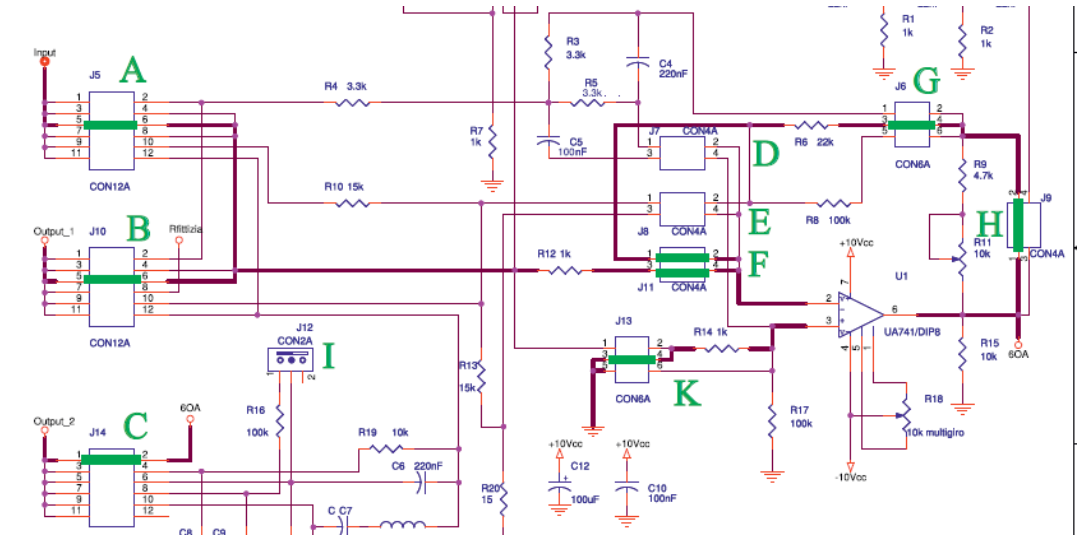
\includegraphics[width=1\linewidth]{media/schemaCircuitaleuA741.png}
    \caption{Schema circuitale della configurazione in catena chiusa}
    \label{fig:schemaCatenaChiusa}
\end{figure}
\FloatBarrier

Al fine di abilitare la configurazione catena chiusa dell'amplificatore operazionale sono stati utilizzati dei Jumper (tratti spessi in verde) che sono stati posizionati come indicato in figura.
\FloatBarrier
Nel circuito di interesse, la resistenza \(R_6\) (tra ingresso invertente dell’amplificatore ed il pin di uscita) ed \(R_{12}\) (tra ingresso invertente dell’amplificatore ed ingresso dell’amplificatore) determinano il guadagno teorico in catena chiusa dell’amplificatore, che vale:

\[A_{Teorico}=-\frac{R_6}{R_{12}}=-\frac{22 k\Omega}{1 k\Omega}=-22\]

La resistenza \(R_{14}\) posta tra l’ingresso non invertente e massa serve per non collegare direttamente l’ingresso non invertente a massa, ma ad un valore di resistenza prossimo a quello dell’ingresso invertente. La resistenza variabile \(R_{18}\) (da 10 k\(\Omega\)) è di tipo multi-giro e serve a compensare il valore di tensione di offset. Dopo aver ridotto l’offset, e stimato il segnale di ingresso in ampiezza e frequenza, per mezzo del generatore di funzioni si fornisce in ingresso al circuito un segnale sinusoidale. Partendo da questo valore di ampiezza, si varia l’ampiezza del segnale (aumentandola o diminuendola) fino ad ottenere la massima tensione d’uscita picco-picco. Se l’ampiezza del segnale supera il valore massimo, l’amplificatore raggiunge la regione di saturazione.
Invece, la frequenza di taglio teorica \(f_{c_{teorica}}\), si ricava dalla relazione già espressa precedentemente, per cui:

\[f_{c_{teorica}}=\frac{GBWP}{|A|}=45,5kHz\]
\subsection{Strumentazione}
Di seguito è riportata la strumentazione utilizzata per la realizzazione del set-up di questa esperienza di laboratorio.

\subsection*{\textbf{PCB}}
\begin{figure}[h]
    \centering
    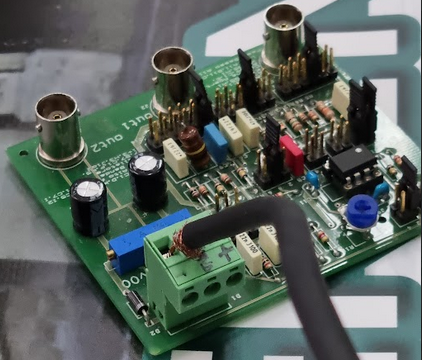
\includegraphics[width=0.5\linewidth]{media/PCB_attacco3pin.png}
    \caption{PCB con attacco a 3 pin per l'alimentazione duale dell'integrato}
    \label{fig:PCB_3pin}
\end{figure}
\FloatBarrier
\subsection*{\textbf{Oscilloscopio Agilent HP 54600B}}
\begin{figure}[h]
    \centering
    \includegraphics[width=0.8\linewidth, height=7cm]{oscilloscopio.png}
    \caption{Oscilloscopio Agilent HP 54600B}
    \label{fig:Agilent HP 54600B}
\end{figure}
\FloatBarrier
\subsection*{\textbf{Generatore di funzioni HP 33120A}}
\begin{figure}[h]
    \centering
    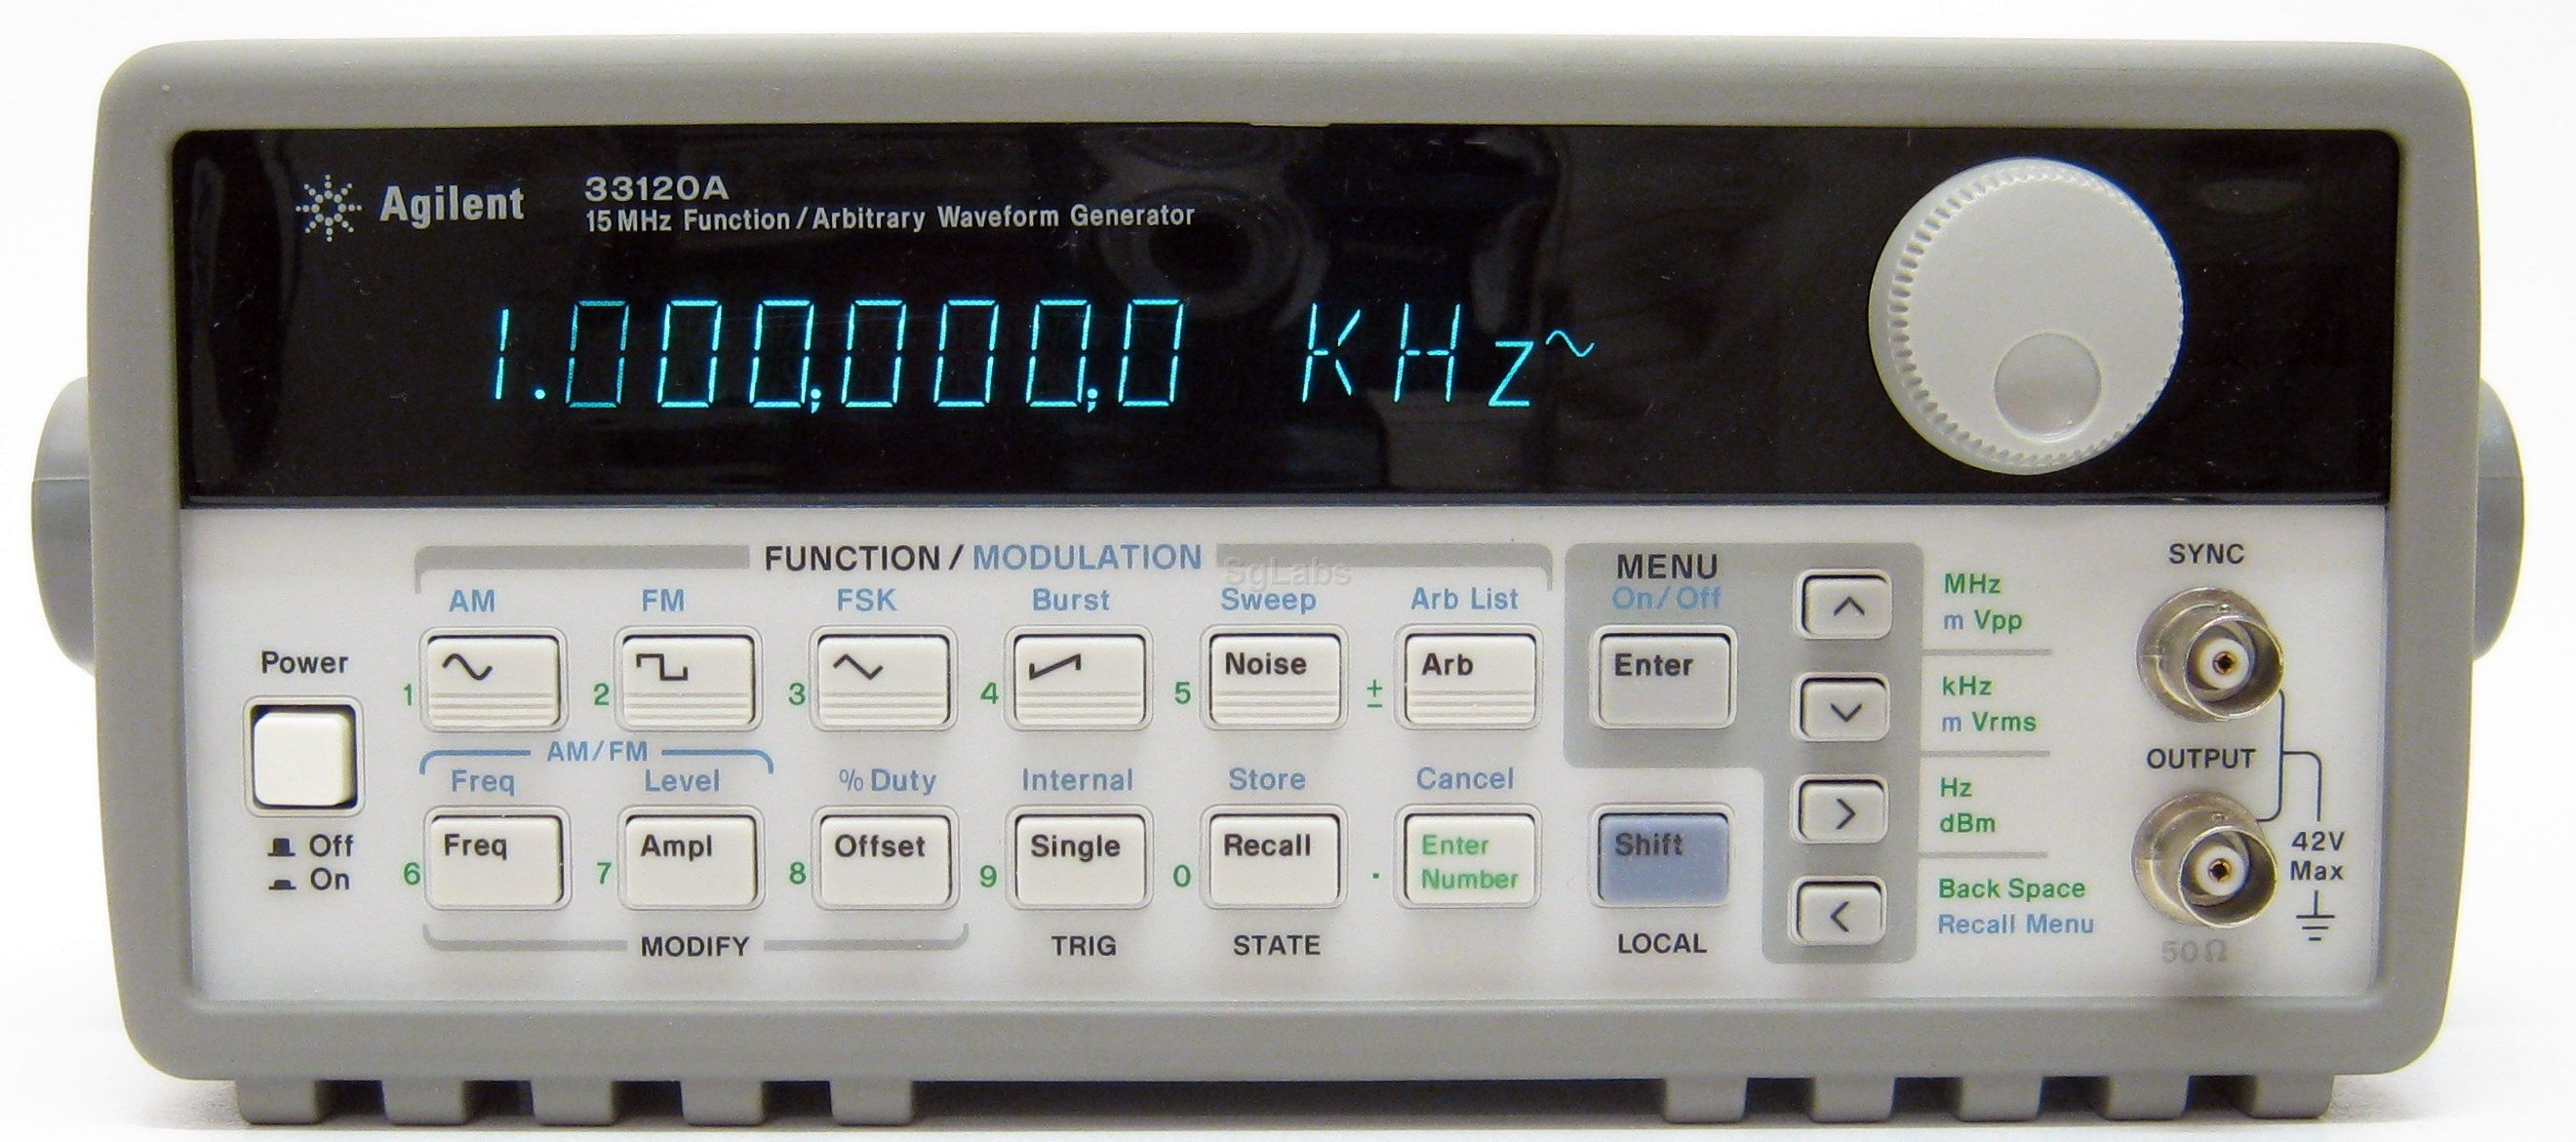
\includegraphics[width=0.9\linewidth, height=6cm]{generatore di funzioni.png}
    \caption{Generatore di funzioni HP 33120A}
    \label{fig:enter-label}
\end{figure}
\FloatBarrier
\subsection*{\textbf{Alimentatore da banco HP E3631A}}
\begin{figure}[h]
    \centering
    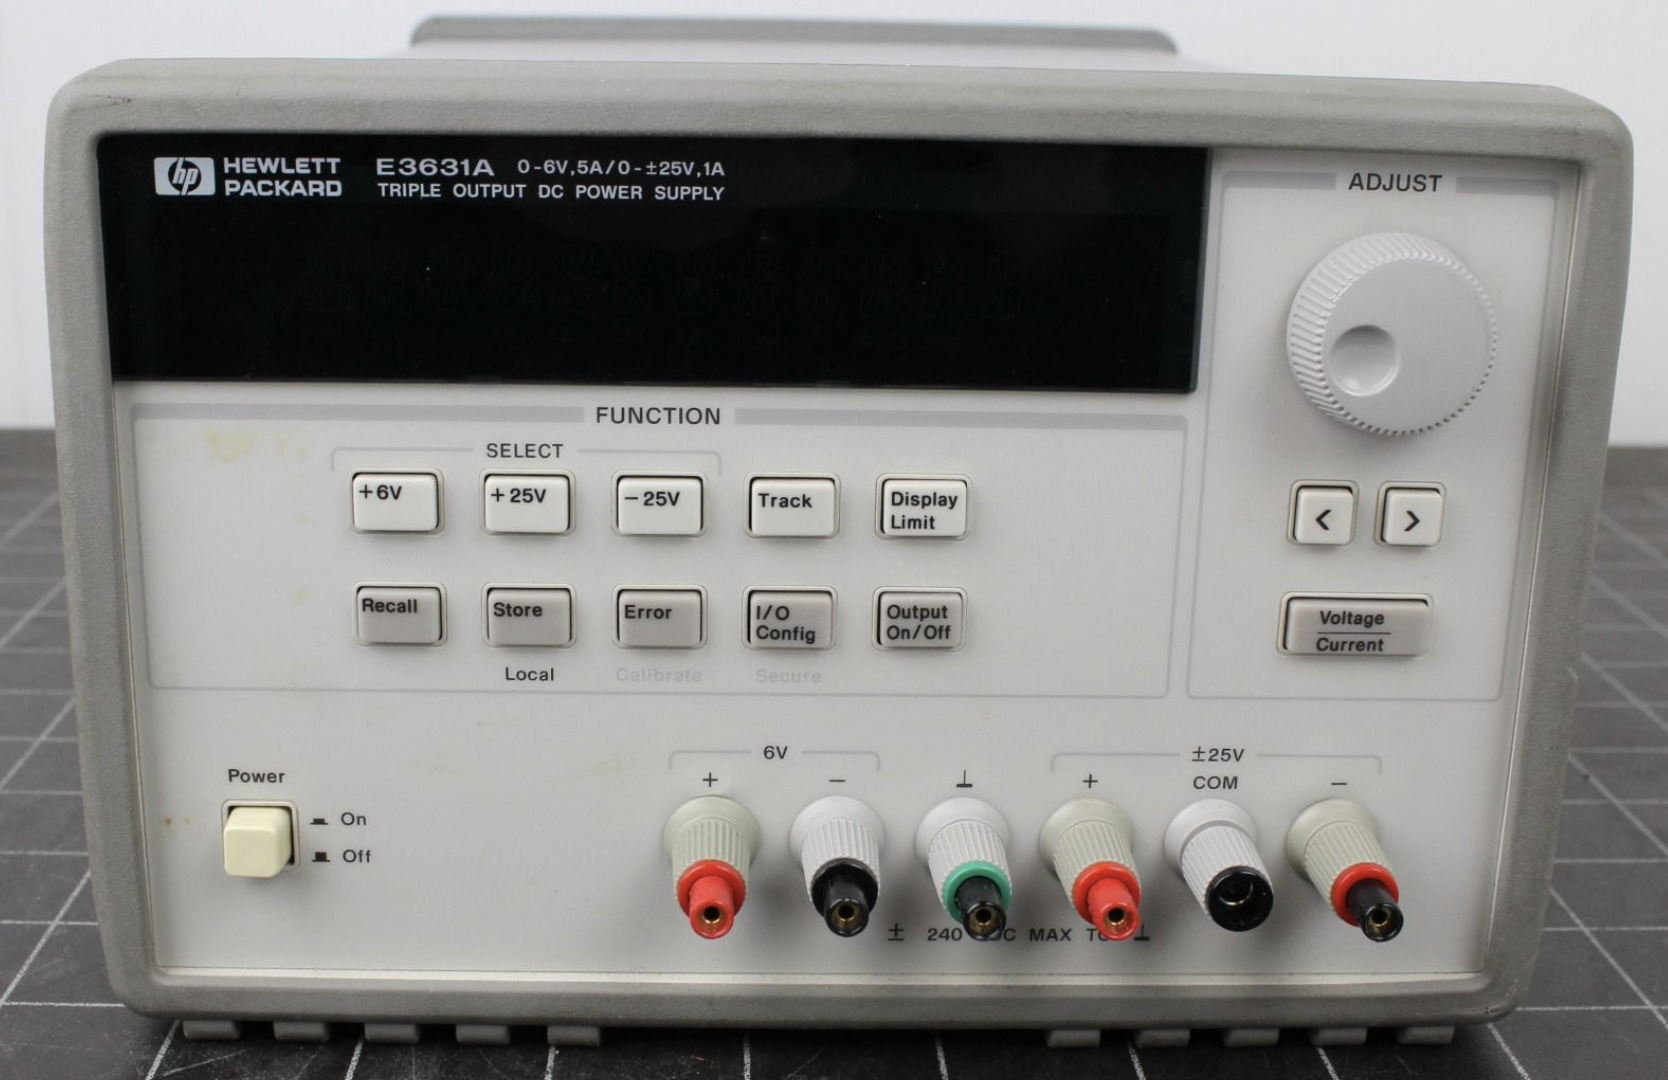
\includegraphics[width=0.8\linewidth, height=7cm]{alimentatore da banco.png}
    \caption{Alimentatore da banco HP E3631A}
    \label{fig:HPE3631A}
\end{figure}
\FloatBarrier
\subsection*{\textbf{Cavi di connessione BNC-BNC}}
\begin{figure}[h]
    \centering
    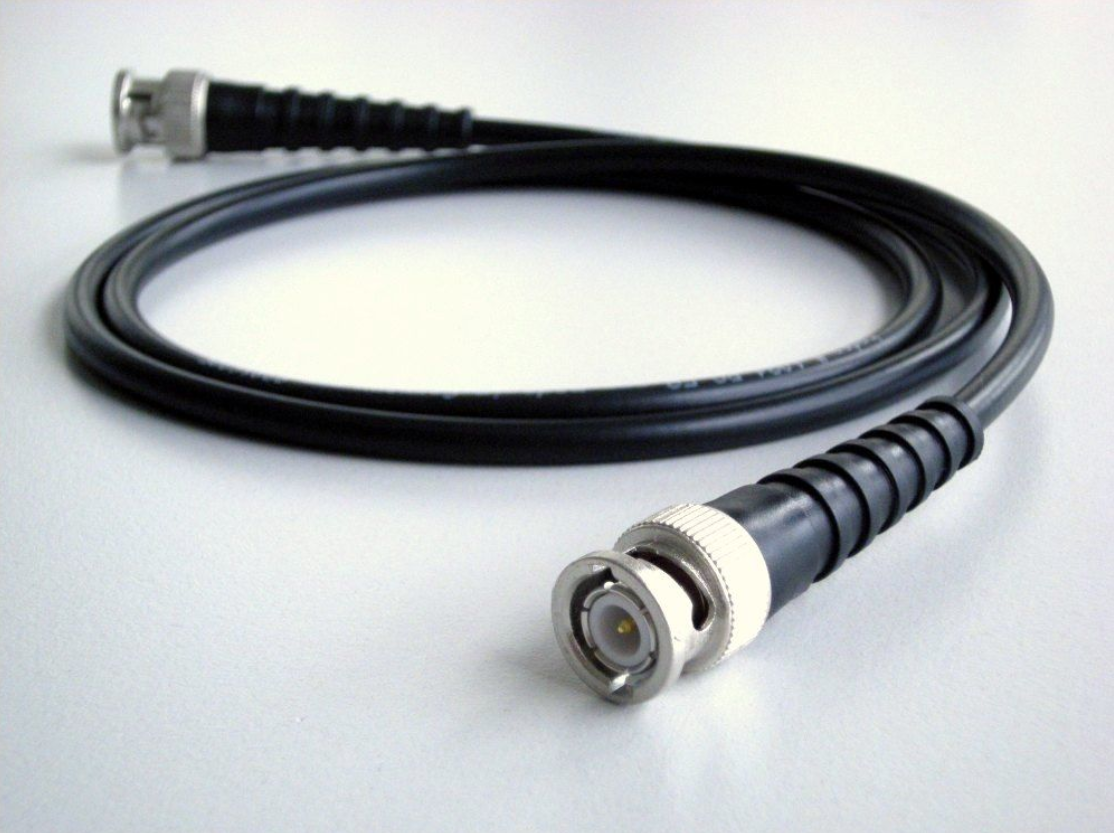
\includegraphics[width=0.75\linewidth]{media/cavoBNC.png}
    \caption{Cavo di connessione BNC-BNC}
    \label{fig:enter-label}
\end{figure}
\FloatBarrier
\clearpage

\subsection{Configurazione della strumentazione per le misurazioni}
Prima di iniziare ad effettuare le misurazioni del caso, abbiamo configurato tutte le strumentazioni a disposizione. Abbiamo dunque:
\begin{itemize}
    \item Collegato i 3 cavi di connessione BNC-BNC e il cavo che permette l'alimentazione dell'integrato secondo la seguente configurazione:
    \begin{itemize}
        \item Uscita del generatore di funzioni Agilent HP 54600B all'ingresso (INPUT) del circuito integrato
        \item  Segnale di ingresso all'operazionale (OUTPUT 1) è stato collegato al canale 1 dell'oscilloscopio
        \item  Segnale di uscita dall'operazionale (OUTPUT 2) è stato collegato al canale 2 dell'oscilloscopio
        \item Uscita COM dell'alimentatore da banco HP E3631A all'ingresso, del circuito integrato, che si trova in altro a destra, facendo riferimento a Figura \ref{fig:PCB_3pin}
    \end{itemize}
    \item Al fine di controllare il corretto funzionamento dell'amplificatore si è impostato sul generatore un segnale di ingresso sinusoidale alla frequenza di $100Hz$ e si è visto come il segnale d'uscita fosse sfasato ed amplificato di all'incirca $20dB$.  
\end{itemize}
\begin{figure}[h]
        \centering
        \includegraphics{PCB_bnc.png}
        \caption{Ingressi/Uscite dell'integrato}
        \label{fig:pcb_bnc}
    \end{figure}
\FloatBarrier
E' importante osservare che l'ampiezza visualizzata sull'oscilloscopio è diversa da quella impostata sul generatore di funzioni a causa del disadattamento di impedenza tra l'oscilloscopio ed il generatore di funzioni.
\begin{itemize}
    \item Avviato l'oscilloscopio su cui visualizzare il segnale d'ingresso dell'operazionale $V_i$ sul canale 1, e il segnale di uscita dell'operazionale $V_o$ sul canale 2.
    Poichè abbiamo utilizzato cavi BNC-BNC e non sonde, abbiamo impostato il valore di \emph{Probe} a 1 mediante l'apposito pulsante posto sotto lo schermo.
    Per migliorare la visualizzazione di entrambi i segnali, abbiamo premuto il pulsante \emph{Auto-Scale}, che permette all'oscilloscopio di visualizzare entrambi i segnali, uno per ognuno della due metà dello schermo.
    
    Ai fini delle misurazioni da effettuare, abbiamo impostato entrambe le forme d'onda sulla linea di 0 V secondo la seguente procedura per entrambi i canali:
    \begin{enumerate}
        \item Selezione del singolo canale dal rispettivo pulsante della sezione verticale
        \item Impostazione del \emph{Coupling} su \textit{Ground} mediante il secondo pulsante posizionato sotto lo schermo
        \item Utilizzo della manopola presente sotto la sezione \textit{Measure} per spostare il riferimento del segnale sulla linea di 0 V
        \item Impostazione del \emph{Coupling} su \textit{AC} mediante il secondo pulsante posizionato sotto lo schermo  
\end{enumerate}
\end{itemize}


\subsection{Misurazioni}
\subsubsection{Calcolo del guadagno e della frequenza di taglio sperimentali}
Per la valutazione sperimentale del guadagno, serve effettuare la stima delle tensioni picco-picco \(V_{o,pp}\)
e \(V_{i, pp}\) attraverso l'utilizzo dell'oscilloscopio. 
Per effettuare ciò, serve impostare il valore della frequenza del segnale d'ingresso dell'integrato sul
generatore di funzioni HP 33120A andando a premere prima il pulsante \textit{Freq} e poi impostando la frequenza da utilizzare, per queste due valutazione è stata scelta \(f=100Hz\). C'è da ricordare che il circuito in questione, è sempre alimentato con una tensione di alimentazione duale pari a ±12V, grazie all'alimentatore da banco HP E3631A precedentemente settato, come scritto nella sottosezione \textbf{\textit{"Tensione di offset e compensazione"}} .  Successivamente, serve regolare opportunamente i valori di KVi e KVo mediante le manopole poste nella sezione verticale dell'oscilloscopio HP 54600B (Figura \ref{fig:Agilent HP 54600B}), in modo da portare il più possibile il segnale visualizzato a schermo, verso il valore di fondo scala. In questo modo, le misure eseguite sono più accurate e viene ridotta l’incertezza di misura. Infine, si va a regolare il valore di Kt mediante l’apposita manopola posta nella sezione orizzontale, sempre dell'oscilloscopio HP 54600B, per avere la visualizzazione di almeno un periodo del segnale di interesse. 
Dopo aver fatto queste regolazioni, si può premere il pulsante \textit{Voltage}, situato nella sezione \textit{Measure} e selezionare per ognuno dei due segnali il tipo di misura, cioè tensione picco-picco \(V_{pp}\), mediante gli appositi pulsanti posizionati sotto lo schermo dell'oscilloscopio. In questo modo i valori di tensione picco-picco di entrambi i segnali vengono automaticamente calcolati dall’oscilloscopio e visualizzati nella parte inferiore dello schermo.
Da queste due stime fornite dall'oscilloscopio, si è ottenuto:

\[V_{o,pp}=4,125V\]

\[V_{i, pp}=190,6mV\]
Da cui:

\[A=-\frac{V_{o,pp}}{V_{i, pp}}=-21,6\]
Andando a determinare quanto vale A, in corrispondenza della frequenza di taglio \(f_c\), tale per cui si ha un'attenuazione di 3dB, segue che:

\[A_{-3dB}=\frac{A}{\sqrt{2}}=-15,27\]
Infine, è possibile calcolare il valore della tensione di uscita in corrispondenza della frequenza di
taglio, facendo uso della relazione:

\[V_o=A_{-3dB} \cdot V_i=2,91V_{pp}\]
Per la valutazione sperimentale della frequenza di taglio, si impostano i due cursori orizzontali dell’oscilloscopio in corrispondenza del valore di tensione \(V_o\) sopra calcolato. Si procede quindi a variare la frequenza del segnale tramite il generatore di funzioni, fino a che il segnale in uscita visualizzato sull’oscilloscopio non risulta tangente ai due cursori orizzontali. In corrispondenza della frequenza di taglio, si può notare che il segnale in uscita è distorto (segnale triangolare) e che il valore di frequenza trovato è diverso dal valore teorico. Questo succede perché si sta lavorando con un segnale di ingresso con ampiezza massima. Per evitare questo effetto, è necessario ridurre l’ampiezza del segnale, ricalcolare il nuovo valore di attenuazione a 3dB e, quindi, stimare la frequenza di taglio. In questo caso, si è trovato che \(f_c=33kHz\).
\clearpage
\subsubsection{Misure di tensione picco-picco}

Per riuscire a ricavare la risposta in frequenza del circuito, è stato necessario ripetere la stessa procedura di misura, lasciando invariate le condizioni operative, per un totale di 24 diversi valori di frequenza.

Per ogni misurazione abbiamo quindi eseguito i seguenti passi:
\begin{enumerate}
    \item Impostato il valore della frequenza del segnale di ingresso del filtro  sul generatore di funzioni, premendo prima il pulsante \emph{Freq} e poi impostando la frequenza desiderata.
    \item Regolato i valori di $K_{V_i}$ e $K_{V_o}$ mediante le manopole poste nella parte superiore della sezione verticale, in modo tale che i segnali si avvicinassero quanto più possibile al valore di fondo scala. In questo modo le misure eseguite sono più accurate e viene ridotta l'incertezza di misura.
    \item Premuto il pulsante \emph{Voltage}, situato nella sezione \emph{Measure} e selezionato per ognuno dei due segnali il tipo di misura, cioè tensione picco-picco $V_{pp}$, mediante gli appositi pulsanti posizionati sotto lo schermo.
    In questo modo i valori di tensione picco-picco di entrambi i segnali $V_i$ e $V_o$ vengono automaticamente calcolati dall'oscilloscopio e visualizzati nella parte inferiore dello schermo.

Di seguito una tabella con i risultati delle misurazioni effettuate:
    
\end{enumerate}
\begin{table}[!ht]
    \centering
    \begin{tabular}{|c|c|c|c|c|c|}
    \hline

        \textbf{FREQ [Hz]} & $\bm{V_i(mV)}$ & $\bm{KV_i(mV)}$ & $\bm{V_o(mV)}$ & $\bm{KV_o(mV)}$ & \textbf{A} \\ \hline

      
        100 & 190,6 & 50 & 4156,0 & 1000 & 21,805  \\ \hline
        1000 & 190,6 & 50 & 4125,0 & 1000 & 21,642  \\ \hline
        10000 & 192,2 & 50 & 3969,0 & 1000 & 20,650 \\ \hline
        15000 & 190,2 & 50 & 3797,0 & 500 & 19,755  \\ \hline
        20000 & 193,8 & 50 & 3578,0 & 500 & 18,462 \\ \hline
        25000 & 193,8 & 50 & 3328,0 & 500 & 17,172  \\ \hline
        30000 & 193,8 & 50 & 3094,0 & 500 & 15,965  \\ \hline
        35000 & 195,3 & 50 & 2884,0 & 500 & 14,767  \\ \hline
        40000 & 196,9 & 50 & 2625,0 & 500 & 13,332  \\ \hline
        45000 & 196,9 & 50 & 2422,0 & 500 & 12,301  \\ \hline
        50000 & 196,9 & 50 & 2250,0 & 500 & 11,427  \\ \hline
        100000 & 200 & 50 & 1231,0 & 200 & 6,155  \\ \hline
        150000 & 200 & 50 & 843,8 & 200 & 4,219  \\ \hline
        200000 & 200 & 50 & 643,8 & 100 & 3,219  \\ \hline
        250000 & 200 & 50 & 512,5 & 100 & 2,563  \\ \hline
        300000 & 200 & 50 & 431,2 & 100 & 2,156  \\ \hline
        350000 & 200 & 50 & 367,2 & 50 & 1,836	\\ \hline																				
        400000	& 200 & 50 & 321,9 & 50 & 1,610	\\ \hline																			
        450000	& 200	& 50	& 284,4	& 50	& 1,422 \\ \hline													
        500000 &	200 &	50 &	256,2 &	50 &	1,281	\\ \hline							
        550000 &	200 &	50 &	232,8 &	50 &	1,164 \\ \hline																		
        600000 &	200 &	50 &	212,5 &	50 &	1,063	\\ \hline																
        650000 &	200 &	50 &	196,9 &	50 &	0,985 \\ \hline																
        700000 &	200 &	50 &	181,2 &	50 &	0,906	\\ \hline																
        
    \end{tabular}
\end{table}
\FloatBarrier

% scrivere le formuke usate per ricavare incertezze ib ase ai datasheet
% piccolo excursus su cosa sono quei valori
% mettere tabelle di excel


\subsection{Calcolo delle incertezze}
In questo paragrafo si effettuerà sulle misure ottenute la valutazione dell'incertezza di \textbf{tipo B}, basata sull'utilizzo di informazioni note a priori quali le specifiche metrologiche degli strumenti adoperati.

\subsubsection{Misure Dirette}

Le misure dirette effettuate durante l'esperienza di laboratorio sono le seguenti:
\begin{itemize}
    \item \textbf{tensione picco-picco V}
    \item \textbf{frequenza f} dei segnali $V_i$ e $V_o$ 
\end{itemize}


\subsubsection*{Incertezza associata alle misure di tensione picco-picco V}

Dalle specifiche metrologiche di ampiezza dell'oscilloscopio, poichè abbiamo utilizzato i due cursori orizzontali per le misure, consideriamo la \textbf{Dual cursor accuracy}, pari a 
\[vertical \ accuracy \pm 0.4\% \ of full scale\]

dove \textbf{vertical accuracy} per l'oscilloscopio Agilent HP 54600B è pari a 1.9\%, mentre \textbf{full scale} è il fondo scala del dispositivo ed è pari a $y_{FS} = 8 \cdot k_v$, dove 8 sono le divisioni verticali e $k_v$ è la \emph{vertical sensitivity} espressa in V/div.

La \emph{Dual cursor accuracy} sopra riportata deriva dalla formula generale dell'incertezza per una differenza 
\[U(V_1 - V_2) = U_G|V_1 - V_2| + 2U_{inl} + 2U{q}\]

Nel nostro caso, l'incertezza di non linearità integrale $U_{inl}$, è stata conglobata nel termine 1.9\% insieme a $U_G$ incertezza di guadagno. L'incertezza di quantizzazione $2U_q$ è invece pari al termine $\pm 0.4\% \cdot y_{FS}$. L'incertezza di offset $U_O$ non è presente poichè nel caso di differenze di misure l'errore di offset si compensa.

Indicato quindi con $V$ il valore di tensione picco-picco letto, l'\textbf{incertezza di caso peggiore} associata a $V$ è data dalla seguente formula:

\[U_V = \frac{1.9}{100} \cdot |V| + \frac{0.4}{100} \cdot 8 \cdot k_v\]

Da questa formula è possibile poi ricavare l'\textbf{incertezza relativa di caso peggiore}:
\[U_{r,V} = \frac{U_V}{V}\]

Seguono due tabelle contenenti per ogni valore di frequenza: il valore di tensione letto, la vertical sensitivity all'atto della lettura, l'incertezza assoluta di caso peggiore e l'incertezza relativa di caso peggiore.

%due tabelle per Vi e Vo 

\begin{table}[!ht]
    \centering
    \begin{tabular}{|c|c|c|c|c|}
    \hline

        \textbf{FREQ [Hz]} & $\bm{V_i(mV)}$ & $\bm{KV_i(mV)}$ & $\bm{U(V_i)}$ & $\bm{U_r(V_i)}$  \\ \hline

      
100	& 190,6	& 50 &	0,005221 &	0,00002739 \\ \hline
1000	& 190,6 &	50 &	0,005221 &	0,00002739 \\ \hline
10000	& 192,2	& 50 &	0,005252 &	0,00002732 \\ \hline
15000	& 192,2	& 50 &	0,005252 &	0,00002732 \\ \hline
20000	& 193,8 &	50 &	0,005282 &	0,00002726 \\ \hline
25000	& 193,8 &	50 &	0,005282 &	0,00002726 \\ \hline
30000	& 193,8 &	50 &	0,005282 &	0,00002726 \\ \hline
35000	& 195,3 &	50 &	0,005311 &	0,00002719 \\ \hline
40000	& 196,9 &	50 &	0,005341 &	0,00002713 \\ \hline
45000	& 196,9 &	50 &	0,005341 &	0,00002713 \\ \hline
50000	& 196,9	& 50 &	0,005341 &	0,00002713 \\ \hline
100000	& 200	& 50 &	0,005400 &	0,00002700 \\ \hline
150000	& 200	& 50 &	0,005400 &	0,00002700 \\ \hline
200000	& 200	& 50 &	0,005400 &	0,00002700 \\ \hline
250000	& 200	& 50 &	0,005400 &	0,00002700 \\ \hline
300000	& 200	& 50 &	0,005400 &	0,00002700 \\ \hline
350000	& 200	& 50 &	0,005400 &	0,00002700 \\ \hline
400000	& 200	& 50 &	0,005400 &	0,00002700 \\ \hline
450000	& 200	& 50 &	0,005400 &	0,00002700 \\ \hline
500000	& 200	& 50 &	0,005400 &	0,00002700 \\ \hline
550000	& 200	& 50 &	0,005400 &	0,00002700 \\ \hline
600000	& 200	& 50 &	0,005400 &	0,00002700 \\ \hline
650000	& 200	& 50 &	0,005400 &	0,00002700 \\ \hline
700000	& 200	& 50 &	0,005400 &	0,00002700	\\ \hline												
        
    \end{tabular}
\end{table}

\begin{table}[!ht]
    \centering
    \begin{tabular}{|c|c|c|c|c|}
    \hline

        \textbf{FREQ [Hz]} & $\bm{V_o(mV)}$ & $\bm{KV_o(mV)}$ & $\bm{U(V_o)}$ & $\bm{U_r(V_o)}$  \\ \hline

      
100	& 4156,0 &	1000	& 0,1110 &	0,00002670  \\ \hline
1000 & 4125,0 & 1000	& 0,1104 &	0,00002676  \\ \hline
10000 & 3969,0 & 1000	& 0,1074 &	0,00002706  \\ \hline
15000	& 3797,0 &	500	& 0,0881 &	0,00002321  \\ \hline
20000	& 3578,0 &	500	& 0,0840 &	0,00002347  \\ \hline
25000	& 3328,0 &	500	& 0,0792 &	0,00002381  \\ \hline
30000	& 3094,0 &	500	& 0,0748 &	0,00002417  \\ \hline
35000	& 2884,0 &	500	& 0,0708 &	0,00002455  \\ \hline
40000	& 2625,0 &	500	& 0,0659 &	0,00002510  \\ \hline
45000	& 2422,0 &	500	& 0,0620 &	0,00002561  \\ \hline
50000	& 2250,0 &	500	& 0,0588 &	0,00002611  \\ \hline
100000	& 1231,0 &	200	& 0,0298 &	0,00002420  \\ \hline
150000	& 843,8	 &  200	& 0,0224 &	0,00002658  \\ \hline
200000	& 643,8	 & 100	& 0,0154 &	0,00002397  \\ \hline
250000	& 512,5	 & 100 &	0,0129 &	0,00002524  \\ \hline
300000	& 431,2 &	100 &	0,0114 &	0,00002642  \\ \hline
350000	& 367,2	& 50 &	0,0086	& 0,00002336  \\ \hline
400000	& 321,9	& 50 &	0,0077	& 0,00002397  \\ \hline
450000	& 284,4	& 50 &	0,0070	& 0,00002463  \\ \hline
500000	& 256,2	& 50 &	0,0065	& 0,00002525  \\ \hline
550000	& 232,8	& 50 &	0,0060	& 0,00002587   \\ \hline
600000	& 212,5	& 50 &	0,0056	& 0,00002653  \\ \hline
650000	& 196,9	& 50 &	0,0053	& 0,00002713  \\ \hline
700000	& 181,2	& 50 &	0,0050	& 0,00002783		 \\ \hline									
        
    \end{tabular}
\end{table}

\clearpage
\subsubsection{Misure Indirette}

L'unica misura indiretta eseguita è il \textbf{guadagno A}.

\subsubsection*{Incertezza associata alle misure del guadagno $A$}

Ricordiamo che il guadagno $A$ dell'amplificatore operazionale è definito come
\[A = \frac{V_o}{V_i}\]
cioè è data dal rapporto di due misure dirette. Pertanto, per poter stimare l'incertezza di $A$, occorre ricorrere alla \textit{formula di propagazione delle incertezze di caso peggiore}:
\[U = \sum_{n=1}^{N} \left|\frac{\partial f}{\partial y_i}\right| \cdot U_i\]

Dall'applicazione di tale formula, nel caso di rapporto tra misure, si ha che l'\textbf{incertezza relativa} è data dalla \textbf{somma delle incertezze relative} delle singole misure dirette. Pertanto nel nostro caso essa è pari a:

\[U_{r,A} = U_{r,V_o} + U_{r,V_i}\]

da cui si ha\textbf{ l'incertezza assoluta di caso peggiore}:

\[U_A = A \cdot U_{r,A}\]

Solitamente i valori di guadagno $A$ vengono riportati in dB(decibel) secondo la formula:

\[A_{dB} = 20\cdot \log_{10} A\]

Applicando la formula di propagazione dellle incertezze si ottiene l'espressione per l'\textbf{incertezza assoluta di caso peggiore} $U_{A_{db}}$:

\[U_{A_{db}} = \frac{20}{\ln 10} \cdot U_{r,A}\]

Segue la tabella riportante per ogni valore di frequenza: il valore calcolato di $A$ con relativa incertezza (assoluta e relativa) di caso peggiore e il valore in dB di $A$ con relativa incertezza assoluta di caso peggiore


\begin{table}[!ht]
    \centering
    \begin{tabular}{|c|c|c|c|c|c|c|}
    \hline
        \textbf{f (Hz)} & \textbf{A} & \textbf{U(A)} & $\bm{U_r(A)}$ & $\bm{A_{dB}}$ & $\bm{U(A_{dB})}$ & $\bm{U_r(A_{dB})}$ \\ \hline
        100 & 21,805 & 0,001180 & 0,0000541 & 26,771 & 0,000470 & 0,0000176 \\ \hline
        1000 & 21,642 & 0,001172 & 0,0000542 & 26,706 & 0,000470 & 0,0000176 \\ \hline
        10000 & 20,650 & 0,001123 & 0,0000544 & 26,299 & 0,000472 & 0,0000180 \\ \hline
        15000 & 19,755 & 0,000998 & 0,0000505 & 25,914 & 0,000439 & 0,0000169 \\ \hline
        20000 & 18,462 & 0,000937 & 0,0000507 & 25,326 & 0,000441 & 0,0000174 \\ \hline
        25000 & 17,172 & 0,000877 & 0,0000511 & 24,697 & 0,000444 & 0,0000180 \\ \hline
        30000 & 15,965 & 0,000821 & 0,0000514 & 24,063 & 0,000447 & 0,0000186 \\ \hline
        35000 & 14,767 & 0,000764 & 0,0000517 & 23,386 & 0,000449 & 0,0000192 \\ \hline
        40000 & 13,332 & 0,000696 & 0,0000522 & 22,498 & 0,000454 & 0,0000202 \\ \hline
        45000 & 12,301 & 0,000649 & 0,0000527 & 21,799 & 0,000458 & 0,0000210 \\ \hline
        50000 & 11,427 & 0,000608 & 0,0000532 & 21,159 & 0,000462 & 0,0000219 \\ \hline
        100000 & 6,155 & 0,000315 & 0,0000512 & 15,785 & 0,000445 & 0,0000282 \\ \hline
        150000 & 4,219 & 0,000226 & 0,0000536 & 12,504 & 0,000465 & 0,0000372 \\ \hline
        200000 & 3,219 & 0,000164 & 0,0000510 & 10,154 & 0,000443 & 0,0000436 \\ \hline
        250000 & 2,563 & 0,000134 & 0,0000522 & 8,173 & 0,000454 & 0,0000555 \\ \hline
        300000 & 2,156 & 0,000115 & 0,0000534 & 6,673 & 0,000464 & 0,0000695 \\ \hline
        350000 & 1,836 & 0,000092 & 0,0000504 & 5,277 & 0,000437 & 0,0000829 \\ \hline
        400000 & 1,610 & 0,000082 & 0,0000510 & 4,134 & 0,000443 & 0,0001071 \\ \hline
        450000 & 1,422 & 0,000073 & 0,0000516 & 3,058 & 0,000448 & 0,0001466 \\ \hline
        500000 & 1,281 & 0,000067 & 0,0000522 & 2,151 & 0,000454 & 0,0002110 \\ \hline
        550000 & 1,164 & 0,000062 & 0,0000529 & 1,319 & 0,000459 & 0,0003482 \\ \hline
        600000 & 1,063 & 0,000057 & 0,0000535 & 0,527 & 0,000465 & 0,0008830 \\ \hline
        650000 & 0,985 & 0,000053 & 0,0000541 & -0,136 & 0,000470 & -0,0034649 \\ \hline
        700000 & 0,906 & 0,000050 & 0,0000548 & -0,857 & 0,000476 & -0,0005554 \\ \hline
    \end{tabular}
\end{table}

\section{Diagramma di Bode del guadagno}
Nella figura ~\ref{fig:Bode} è possibile vedere graficati i valori del guadagno A\textsubscript{dB} rispetto ai valori di frequenza in scala logaritmica, ossia il diagramma di Bode del guadagno dell'OP-AMP. 

% Diagramma di Bode del guadagno dell'OP-AMP
\begin{figure}
    \centering
    \resizebox{0.80\textwidth}{!}{%
    \begin{tikzpicture}
        \begin{axis}
            [xlabel={Decadi di frequenza}, ylabel={A\textsubscript{dB}}, 
            xtick={2,3,4,5,6,7}, xticklabels={$10^2$, $10^3$, $10^4$, $10^5$, $10^6$, $10^7$}]
            \addplot[red, mark=*, only marks,  error bars/.cd, y fixed, y dir=both, y explicit] 
            table[x=x, y=y,y error=error, col sep=comma] {media/bode/bode_adb_logf_u.txt};
        \end{axis}
    \end{tikzpicture}
    }%
    \caption{Diagramma di Bode del guadagno}
    \label{fig:Bode}
\end{figure}



    
    

    
    % blank page
    \newpage
    \mbox{}
    \thispagestyle{empty}
\end{document}
